%% abtex2-modelo-trabalho-academico.tex, v<VERSION> laurocesar
%% Copyright 2012-<COPYRIGHT_YEAR> by abnTeX2 group at http://www.abntex.net.br/
%%
%% This work may be distributed and/or modified under the
%% conditions of the LaTeX Project Public License, either version 1.3
%% of this license or (at your option) any later version.
%% The latest version of this license is in
%%   http://www.latex-project.org/lppl.txt
%% and version 1.3 or later is part of all distributions of LaTeX
%% version 2005/12/01 or later.
%%
%% This work has the LPPL maintenance status `maintained'.
%%
%% The Current Maintainer of this work is the abnTeX2 team, led
%% by Lauro César Araujo. Further information are available on
%% http://www.abntex.net.br/
%%
%% This work consists of the files abntex2-modelo-trabalho-academico.tex,
%% abntex2-modelo-include-comandos and abntex2-modelo-references.bib
%%

% ------------------------------------------------------------------------
% ------------------------------------------------------------------------
% abnTeX2: Modelo de Trabalho Academico (tese de doutorado, dissertacao de
% mestrado e trabalhos monograficos em geral) em conformidade com
% ABNT NBR 14724:2011: Informacao e documentacao - Trabalhos academicos -
% Apresentacao
% ------------------------------------------------------------------------
% ------------------------------------------------------------------------

\documentclass[
	% -- opções da classe memoir --
	12pt,				% tamanho da fonte
	openright,			% capítulos começam em pág ímpar (insere página vazia caso preciso)
	twoside,			% para impressão em recto e verso. Oposto a oneside
	a4paper,			% tamanho do papel.
	% -- opções da classe abntex2 --
	%chapter=TITLE,		% títulos de capítulos convertidos em letras maiúsculas
	%section=TITLE,		% títulos de seções convertidos em letras maiúsculas
	%subsection=TITLE,	% títulos de subseções convertidos em letras maiúsculas
	%subsubsection=TITLE,% títulos de subsubseções convertidos em letras maiúsculas
	% -- opções do pacote babel --
	english,			% idioma adicional para hifenização
	french,				% idioma adicional para hifenização
	spanish,			% idioma adicional para hifenização
	brazil				% o último idioma é o principal do documento
	]{abntex2}

% ---
% Pacotes básicos
% ---
\usepackage{lmodern}			% Usa a fonte Latin Modern
\usepackage[utf8]{inputenc}		% Codificacao do documento (conversão automática dos acentos)
\usepackage[T1]{fontenc}		% Selecao de codigos de fonte.
\usepackage{lastpage}			% Usado pela Ficha catalográfica
\usepackage{indentfirst}		% Indenta o primeiro parágrafo de cada seção.
\usepackage{color}				% Controle das cores
\usepackage{graphicx}			% Inclusão de gráficos
\usepackage{float}				% Habilitar opção H nos elementos
\usepackage{microtype} 			% para melhorias de justificação
% ---
% Adicionado por Madson Dias
% ---

\usepackage{utils/ifce-modelo} 					% Pacote com informações da customização
\usepackage{utils/ifce-facilitadores} 					% Pacote com facilitadore 
\graphicspath{ {figuras/graficos/} {figuras/imagens/}}  % Inclusão dos paths para imagens
\usepackage{xstring} 									% Criar comandos com IF
\usepackage{caption}
\usepackage{subcaption}
%\usepackage[portuguese, ruled, linesnumbered]{utils/algorithm2e}
\usepackage{amsmath}
\usepackage{algorithm}
\usepackage[noend]{algpseudocode}
%\makeatletter
\def\BState{\State\hskip-\ALG@thistlm}
\renewcommand{\ALG@name}{Algoritmo}
\renewcommand{\listalgorithmname}{Lista de \ALG@name s}
\makeatother

% Declaracoes em Português
\algrenewcommand\algorithmicend{\textbf{fim}}
\algrenewcommand\algorithmicdo{\textbf{faça}}
\algrenewcommand\algorithmicwhile{\textbf{enquanto}}
\algrenewcommand\algorithmicfor{\textbf{para}}
\algrenewcommand\algorithmicif{\textbf{se}}
\algrenewcommand\algorithmicthen{\textbf{então}}
\algrenewcommand\algorithmicelse{\textbf{senão}}
\algrenewcommand\algorithmicreturn{\textbf{devolve}}
\algrenewcommand\algorithmicfunction{\textbf{função}}



\algrenewcommand\algorithmicforall{\textbf{para todo}}
\algrenewcommand\algorithmicloop{\textbf{loop}}
\algrenewcommand\algorithmicrepeat{\textbf{repetir}}
\algrenewcommand\algorithmicuntil{\textbf{até}}
\algrenewcommand\algorithmicprocedure{\textbf{procedimento}}
\algrenewcommand\algorithmicrequire{\textbf{Exige:}}
\algrenewcommand\algorithmicensure{\textbf{Garante:}}
\newcommand{\Not}{\textbf{não }}





% Rearranja os finais de cada estrutura
%\algrenewtext{Procedure}{\textbf{Procedimento~} }
\algrenewtext{goto}{\textbf{vai para~} }
\algrenewtext{EndWhile}{\algorithmicend\ \algorithmicwhile}
\algrenewtext{EndFor}{\algorithmicend\ \algorithmicfor}
\algrenewtext{EndIf}{\algorithmicend\ \algorithmicif}
\algrenewtext{EndFunction}{\algorithmicend\ \algorithmicfunction}

% O comando For, a seguir, retorna 'para #1 -- #2 até #3 faça'
\algnewcommand\algorithmicto{\textbf{até}}
\algrenewtext{For}[3]%
{\algorithmicfor\ #1 $\gets$ #2 \algorithmicto\ #3 \algorithmicdo}
\setlist[itemize]{noitemsep, topsep=0pt, leftmargin=1.75cm}





% ---
% Pacotes adicionais, usados apenas no âmbito do Modelo Canônico do abnteX2
% ---
\usepackage{lipsum}				% para geração de dummy text
% ---

% ---
% Pacotes de citações
% ---
\usepackage[brazilian,hyperpageref]{backref}	 % Paginas com as citações na bibl
\usepackage[alf]{abntex2cite}	% Citações padrão ABNT
\usepackage[table,xcdraw]{xcolor}
% ---
% CONFIGURAÇÕES DE PACOTES
% ---

% ---
% Configurações do pacote backref
% Usado sem a opção hyperpageref de backref
\renewcommand{\backrefpagesname}{Citado na(s) página(s):~}
% Texto padrão antes do número das páginas
\renewcommand{\backref}{}
% Define os textos da citação
\renewcommand*{\backrefalt}[4]{
	\ifcase #1 %
		Nenhuma citação no texto.%
	\or
		Citado na página #2.%
	\else
		Citado #1 vezes nas páginas #2.%
	\fi}%
% ---

% ---
% Informações de dados para CAPA e FOLHA DE ROSTO
% ---
% Informações do Autor e do trabalho
% ------------------------------------
\autor{Walber Florêncio de Almeida}
\titulo{Tratando Erros em TLBs de Instruções Utilizando um Método de Paridade Simples}
\linha{Sistemas de Computação} % Inteligência Artificial, Computação aplicada ou Engenharia de Software

\orientador{Dr. Otávio Alcântara de Lima Júnior}
%\coorientador{<Nome do Coorientador>} % Se você tem um coorientador, descomente esta linha

% Professores convidados para a banca
% ------------------------------------
% 
%  - Caso tenha um terceiro professor convidado, remova os comentários

\nomeprofessorA{Dr. Thiago Alves Rocha}
\instituicaoprofessorA{Instituto Federal de Educação, Ciência e Tecnologia do Ceará (IFCE)}

\nomeprofessorB{Dr. Corneli Gomes Furtado Junior}
\instituicaoprofessorB{Instituto Federal de Educação, Ciência e Tecnologia do Ceará (IFCE)}

%\nomeprofessorC{<Nome do Professor C>}
%\instituicaoprofessorC{<Instituição do Professor C> (<Sigla C>)}

% ---


% ---
% Configurações de aparência do PDF final

% alterando o aspecto da cor azul
\definecolor{blue}{RGB}{0,0,0}

% informações do PDF
\makeatletter
\hypersetup{
     	%pagebackref=true,
		pdftitle={\@title},
		pdfauthor={\@author},
    	pdfsubject={\imprimirpreambulo},
	    pdfcreator={LaTeX with abnTeX2},
		pdfkeywords={abnt}{latex}{abntex}{abntex2}{trabalho acadêmico},
		colorlinks=true,       		% false: boxed links; true: colored links
    	linkcolor=blue,          	% color of internal links
    	citecolor=blue,        		% color of links to bibliography
    	filecolor=magenta,      		% color of file links
		urlcolor=blue,
		bookmarksdepth=4
}
\makeatother
% ---

% ---
% Espaçamentos entre linhas e parágrafos
% ---

% O tamanho do parágrafo é dado por:
\setlength{\parindent}{1.3cm}

% Controle do espaçamento entre um parágrafo e outro:
\setlength{\parskip}{0.2cm}  % tente também \onelineskip

% ---
% compila o indice
% ---
\makeindex
% ---

% ----
% Início do documento
% ----
\begin{document}

% Seleciona o idioma do documento (conforme pacotes do babel)
%\selectlanguage{english}
\selectlanguage{brazil}

% Retira espaço extra obsoleto entre as frases.
\frenchspacing

% ----------------------------------------------------------
% ELEMENTOS PRÉ-TEXTUAIS
% ----------------------------------------------------------
% \pretextual
\imprimircapa % Capa *
\imprimirfolhaderosto % Folha de rosto *

\begin{folhadeaprovacao}

    \begin{center}
    
\includegraphics[width=2.5cm]{brasao_republica.jpg} \\
    \vspace{.5cm}
    {\ABNTEXchapterfont\large\imprimirinstituicao}
    \vspace{1cm}

    {\ABNTEXchapterfont\large\imprimirautor}

    % \vspace*{\fill}\vspace*{\fill}
    % \begin{center}
    %   \ABNTEXchapterfont\bfseries\Large\imprimirtitulo
    % \end{center}
    %\vspace*{\fill}
    
    %\hspace{.45\textwidth}
    % \begin{minipage}{.5\textwidth}
    %     \imprimirpreambulo
    %     {\large\imprimirdata}
    % \end{minipage}%
    %\vspace*{\fill}
   \end{center}
   Esta qualificação foi julgada adequada para aprovação pela Coordenação do Programa de Pós-Graduação em Ciência
da Computação do Instituto Federal de Educação, Ciência e Tecnologia do Ceará e pela banca
examinadora:

\vfill

  \begin{center}
  \begin{minipage}{10cm}
   \assinatura{\textbf{\imprimirorientadorRotulo~\imprimirorientador} \\ Instituto Federal de Educação, Ciência e Tecnologia do Ceará (IFCE)}

   \if \imprimircoorientador
    
   \else
    \assinatura{\textbf{\imprimircoorientadorRotulo~\imprimircoorientador}  \\ Instituto Federal de Educação, Ciência e Tecnologia do Ceará (IFCE)}
   \fi

   \if \nomeprofessorA \instituicaoprofessorA
    
   \else
    \assinatura{\textbf{\imprimirnomeprofessorA}  \\ \imprimirinstituicaoprofessorA}
   \fi

   \if \nomeprofessorB
    
   \else
    \assinatura{\textbf{\imprimirnomeprofessorB}  \\ \imprimirinstituicaoprofessorB}
   \fi
   
   \if \nomeprofessorC
    
   \else
    \assinatura{\textbf{\imprimirnomeprofessorC}  \\ \imprimirinstituicaoprofessorC}
   \fi
  \end{minipage}

  \end{center} 
  \vfill
   %\assinatura{\textbf{Professor}  \\ Instituto Federal do Ceará (IFCE)}
      
   \begin{center}
    \vspace*{\fill}
    {\large\imprimirlocal}
    \par
    {\large\imprimirdata}
    \vspace*{1cm}
  \end{center}
  
\end{folhadeaprovacao}


%\includepdf{pretextual/folhadeaprovacao.pdf} 	% Folha de aprovação (Depois da apresentação)
%\begin{dedicatoria}
   \vspace*{\fill}
   \centering
   \noindent
   \textit{ Este trabalho é dedicado às crianças adultas que,\\
   quando pequenas, sonharam em se tornar cientistas.} \vspace*{\fill}
\end{dedicatoria} 				% Dedicatória
%\begin{agradecimentos}
Os agradecimentos principais são direcionados à Gerald Weber, Miguel Frasson,
Leslie H. Watter, Bruno Parente Lima, Flávio de Vasconcellos Corrêa, Otavio Real
Salvador, Renato Machnievscz\footnote{Os nomes dos integrantes do primeiro
projeto abn\TeX\ foram extraídos de
\url{http://codigolivre.org.br/projects/abntex/}} e todos aqueles que
contribuíram para que a produção de trabalhos acadêmicos conforme
as normas ABNT com \LaTeX\ fosse possível.

Agradecimentos especiais são direcionados ao Centro de Pesquisa em Arquitetura
da Informação\footnote{\url{http://www.cpai.unb.br/}} da Universidade de
Brasília (CPAI), ao grupo de usuários
\emph{latex-br}\footnote{\url{http://groups.google.com/group/latex-br}} e aos
novos voluntários do grupo
\emph{\abnTeX}\footnote{\url{http://groups.google.com/group/abntex2} e
\url{http://www.abntex.net.br/}}~que contribuíram e que ainda
contribuirão para a evolução do \abnTeX.

\end{agradecimentos} 			% Agradecimento
%\begin{epigrafe}
    \vspace*{\fill}
	\begin{flushright}
		\textit{%
		``<Citação Célebre>''\\
		(<Autor da citação>)}
	\end{flushright}
\end{epigrafe} 				% Epígrafe
\setlength{\absparsep}{18pt} % ajusta o espaçamento dos parágrafos do resumo
\begin{resumo}
 Para entrar em estado de execução, programas podem solicitar ao sistema operacional o espaço de memória que necessitam. A eles é dado espaço de memória virtual, cujos endereços são chamados de páginas. Quem gerencia essas páginas e converte endereços virtuais em endereços físicos da memória é o \textit{Memory Manegement Unit} (MMU). Dentro do MMU, fica a \textit{translation lookaside buffer} (TLB), uma cache que armazena apenas as páginas mais referenciadas. As entradas de uma TLB podem ser afetadas por interferências nas células de memória, conhecidas como \textit{Multiple Cell Upset} (MCU). Uma das consequências causadas pelos MCUs em TLBs é o aumento da necessidade de tratamento de falta de página, o que interfere diretamente no desempenho do sistema. No entanto, falhas ainda mais graves podem acontecer, como o congelamento do sistema ou corrupção de dados. Diferentes métodos para proteger TLBs foram propostos ao longo dos anos, no entanto, muitas dessas soluções requerem mais espaço de memória ou poder computacional, sobrecarregando o sistema. Nesse contexto, códigos de detecção de erros que se apropriam do princípio da localidade e que não adicionam bits de redundância, permitem reduzir ou até mesmo evitar o impacto destas falhas. Essa codificação envolve manipular os bits do endereço de memória, aumentando a distância Hamming entre endereços próximos através do cálculo de paridade entre os bits pares e ímpares, individualmente. O resultado destas paridades é alocado nos dois bits mais significativos (MSBs) do endereço, enquanto os outros bits permanecem inalterados. Este trabalho propõe explorar ainda mais o princípio da localidade, fazendo o cálculo das paridades com parcelas menores de bits ao invés de usar toda a palavra. Este método propaga o erro apenas dos bits menos significativos, que é onde a ocorrência de erros pode gerar falhas mais graves. Foram propostos quatro cenários: calculando a paridade entre os 4, 8, 12 e 16 bits menos significativos, num endereço com 32 bits. Foram realizadas 10 mil iterações para cada tipo de falha (única, dupla e tripla adjacente) nos experimentos com injeção de falha pseudoaleatória em cada cenário, inseridas em diferentes posições e endereços a cada execução. O \textit{benchmark} era composto pelos \textit{traces} de memória de algoritmos de aplicações reais. O simulador de TLB implementado apresenta o LRU como política de substituição e 8 posições de memória. Após os experimentos, ficou indicado que proteger os bits menos significativos no cálculo  de paridade apresentou resultados semelhantes a proteger a palavra toda, ocupando até 20\%\ de portas XOR. Além disso, ainda reduz bastante as falhas protegendo apenas os 4-LSBs, confirmando que é possível proteger a TLB ocupando menos área na síntese do circuito. 

 \textbf{Palavras-chave}: códigos de correção de erros. \textit{multiple cell upsets. translation lookaside buffer}.
\end{resumo} 					% Resumo em português
\begin{resumo}[Abstract]
 \begin{otherlanguage*}{english}
   Programs can request the memory space needed to run to the operating system.
   They receive virtual memory space, with addresses called pages. The Memory Management Unit (MMU) is responsible for managing the pages and converting these virtual addresses into physical memory addresses. Inside the MMU is located the Translation Lookaside Buffer (TLB), a cache memory that stores only the most referenced pages. Interferences known as Multiple Cell Upsets (MCUs) can affect TLB entries’ memory cells. An MCU occurrences consequence in TLBs is the higher necessity of page fault handling, which directly interferes with the system’s performance. However, even serious faults might happen, like system freezing or data corruption. To protect TLBS, different methods have been proposed over the years, including parity techniques and spatial redundancy, but many of these solutions require more memory space or computational power, overloading the system. In this context, an error correction code (ECC) that approves the principle of locality and does not add redundancy bits, reduces those failures’ impacts. This coding involves manipulating the memory address’ bits, enhancing the Hamming distance between near addresses through parity calculation between even and odd bits. The result of these calculations is allocated in the two most significant bits (MSBs) of the address, while the other bits remain unchanged. This paper proposes to explore even more the principle of locality, calculating the parities of minor sections of bits instead of using the entire word.This method only propagates the error of the least significant bits (LSBs), where the occurrence of errors may result in serious failures. This work proposed four scenarios: calculating the parity among the 4, 8, 12, and 16 LSBs in a 32-bit address. There were running ten thousand iterations to each kind of failure (single, double adjacent, and triple adjacent) in the experiments, with pseudorandom failure injection in each scenario, inserted in different positions and addresses on each iteration. Algorithm memory traces from real applications composed the benchmark of the experiments. The implemented TLB simulator uses the Least Recently Used (LRU) substitution policy and eight memory positions. After the experiments, it was indicated that protecting the less significant bits in parity calculation showed similar results to protecting the entire word, occupying up to 20\%\ of XOR gates. Futhermore, it also greatly reduces failures by protecting only the 4-LSBs, confirming that it is possible to protect the TLB by occupying less area in the synthesis of the circuit.
   \vspace{\onelineskip}
 
   \noindent 
   \textbf{Keywords}: error correction codes. multiple cell upsets. translation lookaside buffer.
 \end{otherlanguage*}
\end{resumo} 				% Resumo em inglês
% inserir lista de ilustrações
\pdfbookmark[0]{\listfigurename}{lof}
\listoffigures*
\cleardoublepage
% inserir lista de tabelas
\pdfbookmark[0]{\listtablename}{lot}
\listoftables*
\cleardoublepage
% ---
% inserir lista de algoritmos
%\pdfbookmark[0]{\listalgorithmname}{loa}
%\listofalgorithms
%\cleardoublepage
% ---
%\begin{siglas}
  \item[ABNT] Associação Brasileira de Normas Técnicas
  \item[abnTeX] ABsurdas Normas para TeX
\end{siglas}  			% Lista de abreviaturas e siglas
%\begin{simbolos}
\item[$ \oplus $] XOR
\end{simbolos} 				% Lista de símbolos
% inserir o sumario
\pdfbookmark[0]{\contentsname}{toc}
\tableofcontents*
\cleardoublepage
% ---



% ----------------------------------------------------------
% ELEMENTOS TEXTUAIS
% ----------------------------------------------------------
\textual

\chapter{Introdução}\label{cap:introducao}
Os sistemas operacionais alocam programas que estão em execução em endereços
da memória virtual, que são solicitados pelos programas e divididos nas chamadas páginas
virtuais. Quando a memória virtual é usada, esses endereços não são
diretamente colocados no barramento da memória, eles são enviados para a \textit{Memory
Management Unit} (MMU), que é quem mapeia as páginas em endereços físicos da memória principal (RAM) de forma dinâmica, usando as tabelas de páginas.

No entanto, endereços virtuais grandes (por exemplo, os de 32 e 64 bits)
geram tabelas de páginas de tamanho significativo, impactando diretamente no
desempenho do sistema. Com isso, e sabendo que os programas tendem a referenciar alguns campos da paginação com mais frequência, começou-se a usar uma cache que armazena apenas as páginas mais referenciadas, acelerando o processo de conversão. Essa cache é chamada \textit{translation lookaside buffer} (TLB),localiza-se dentro da MMU e pode funcionar como uma \textit{Content-Addressable Memory} (CAM) \cite{griffith2005tlb}.

\section{Problemática}

Os constantes avanços tecnológicos no campo da microeletrônica têm proporcionado dispositivos cada vez menores e mais integrados, o que contribui com a eficiência e a rapidez dos mesmos. No entanto, esse nível de integração dos circuitos torna esses dispositivos mais sensíveis a interferências externas. Quantos mais integrados os circuitos, mais células podem ser atingidas.

Essas interferências podem causar dois tipos de evento: \textit{single event upset} (SEU) e \textit{multiple cells upset} (MCU), que respectivamente acontecem quando um ou múltiplos bits são atingidos \cite{chugg2004broadening}. Quando atingem as entradas de uma TLB, essas falhas podem gerar tratamento de falta de página, o que atrapalha a performance do sistema, e, nos piores casos, falhas mais graves, como congelamento do sistema e corrupção de dados.

Diferentes métodos para proteger as TLBs contra SEUs e MCUs foram propostos ao longo de anos de pesquisa, incluindo técnicas de paridade \cite{griffith2005tlb}, redundância espacial \cite{lang2013processor} e técnicas de correção de erros \cite{sanchez2016combined}, \cite{pagiamtzis2006soft} e \cite{sanchez2012hamming}.No entanto, muitas dessas soluções requerem mais espaço de memória ou poder computacional, sobrecarregando o sistema.

O trabalho em \cite{sanchez2019reducing}
utiliza-se do princípio da localidade, que diz que os endereços referenciados tendem a estar próximos, para proteger TLBs de instruções contra erros adjacentes sem a inclusão de bits de redundância, apenas manipulando os números da página virtual (NPV) com cálculos de paridade.

\section{Objetivo geral e objetivos específicos}

O objetivo deste trabalho é estender a estratégia utilizada por \cite{sanchez2019reducing}, calculando a paridade com grupos menores de NPVs, em diferentes tamanhos, e mostrar os resultados comparando um cenário não protegido, o código original e os esquemas propostos.

Para alcançar esse objetivo, se fazem necessários os objetivos específicos a seguir:

\begin{itemize}
    \item Implementar um simulador de TLB com um método de injeção de falhas pseudoaleatórias;
.    \item Criar um \textit{benchmark} baseado em traces de memória de aplicações reais;
    \item Implementar quatro cenários de códigos: 4-,8-,12-,16-LSB;
    \item Avaliar o desempenho dos códigos propostos em relação a taxa de falsos positivos, bem como o tamanho do circuito em portas XOR.
\end{itemize}

\section{Estrutura do trabalho}

O restante deste trabalho está organizado como segue:

No Capítulo 2, as fundamentações teóricas apontam conhecimentos importantes para o entendimento da pesquisa. Além disso, apresenta uma revisão de trabalhos relacionados, apresentando códigos de correção de erros já propostos com aplicações semelhantes.

No Capítulo 3 é mostrada a metodologia abordada neste trabalho, com passo-a-passo das atividades desenvolvidas e explicação sobre os códigos implementados.

No Capítulo 4, são apresentados e discutidos os resultados preliminares obtidos com os experimentos realizados.

E por fim, no Capítulo 5, um cronograma mensal com a perspectiva de realização de uma lista de atividades que termina com a defesa da dissertação. 				% Capítulo de introdução
\chapter{Fundamentação Teórica}

\label{cap:2}

Neste capítulo serão abordados fundamentos e conceitos relevantes para este trabalho e apresentados trabalhos relacionados. São apresentados os conceitos de memória virtual e TLB. Em seguida, uma breve explicação sobre como ocorrem as falhas causadas por interferências externas. Então, uma seção demonstra quais problemas essas falhas podem causar às TLBs. Também é importante saber como se faz o cálculo da paridade simples e do código Hamming. Por fim, um revisão de trabalhos relacionados é apresentada, comentando sobre códigos de proteção à sistemas de memória e TLBs.

\section{Memória virtual}

Quando um sistema de memória utiliza memória virtual, o tamanho total de um
programa a ser executado podem ser
superiores à quantidade de memória física disponível para ele. O sistema operacional
armazena as partes ativas do programa na RAM e deixa o restante em disco. Quando o
programa entra em estado de execução, as páginas virtuais são transferidas do disco para a
memória principal.

Nessa técnica, o número da página virtual identifica a página virtual que é
associada ao endereço físico, funcionando como um índice na tabela de páginas. A Figura \ref{fig:memory} é uma representação desse esquema. Além dos endereços, a tabela de páginas possui outras informações, como o bit de validade, que indica se
uma página está ou não na memória principal. Se o bit tem valor 0, isto indica que a página
virtual não está na RAM, mas se o valor do bit é igual a 1, a página está na memória
principal \cite{Tannenbaum}.

\begin{figure}[ht]
    \centering
    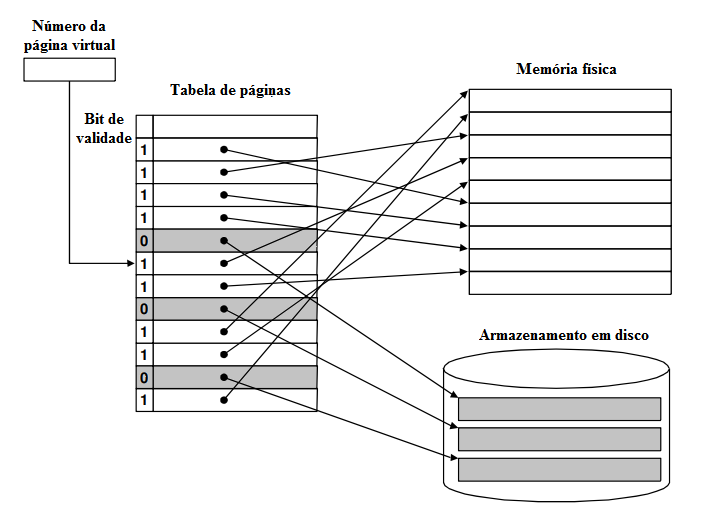
\includegraphics[scale=0.5]{figuras/memoria virtual.PNG}
    \caption{Esquema explicativo da memória virtual}{Fonte: adaptação de \cite{Tannenbaum}}
    \label{fig:memory}
\end{figure}

Sempre que um programa faz referência a um
endereço virtual, o MMU localiza na tabela de páginas o endereço físico correspondente.
Caso a página não esteja na memória, dizemos que ocorreu uma falta de página. Se a RAM
já estiver cheia, o sistema operacional se utiliza de algoritmos de substituição de páginas
para transferir páginas da memória principal para o disco, em seguida busca a página
desejada no disco e transfere para a memória principal.

\section{CAM}

Uma memória do tipo CAM usa um mecanismo de pesquisa e busca de endereços para verificar se as palavras buscadas estão armazenadas na memória. A Figura \ref{fig:cam} mostra como a CAM funciona. Quando uma palavra é buscada, a CAM precisa verificar a compatibilidade de cada bit da palavra com os bits armazenados em suas células de memória. Na entrada de cada célula de memória há um elemento de comparação, que assume os valores zero ou um de acordo com a combinação ou não do bit buscado com o bit armazenado. Como as células estão conectadas em paralelo, o impulso elétrico com os valores buscados chega em todas as células ao mesmo tempo. Então, um elemento chamado \textit{match line} verifica se houve combinação em todos os bits de cada linha, ou seja, se o valor  assumido das combinações foi um e o circuito fecha naquela linha. Se houver, significa que o endereço buscado foi encontrado \cite{maestro2013soft}.

\begin{figure}[ht]
    \centering
    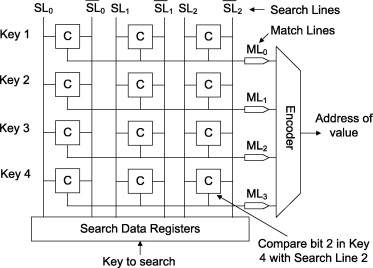
\includegraphics[scale=0.7]{figuras/cam.png}
    \caption{Arquitetura de uma CAM}{Fonte: \cite{maestro2013soft}}
    \label{fig:cam}
\end{figure}

Uma TLB é uma cache normalmente implementada com a arquitetura de uma CAM. Ela serve para acelerar o processo de tradução entre endereços físicos e virtuais. Na seção a seguir, ela será melhor abordada.

\section{TLB}
Nos sistemas de memória que utilizam paginação, as tabelas de páginas são
mantidas dentro da memória principal, devido a suas grandes dimensões, o que interfere
diretamente no desempenho do sistema. A maioria dos programas tende a referenciar mais vezes o mesmo pequeno grupo de páginas virtuais, que vai mudando ao longo da execução.
Sabendo disto, foi criada uma cache que se localiza dentro do MMU, portanto, mais perto
do gerenciador de memória, que armazena apenas as páginas mais referenciadas. A essa
cache foi dada o nome de \textit{translation lookaside buffer}(TLB). A Figura \ref{fig:arq} é uma representação dessa organização. O endereço virtual é buscado na TLB. Caso esteja, acontece um TLB \textit{hit}, dispensando o acesso à tabela de páginas e acelerando o processo de tradução. Caso não esteja na cache, acontece um TLB \textit{miss} e a tabela de páginas é consultada. 

\begin{figure}[ht]
\centering
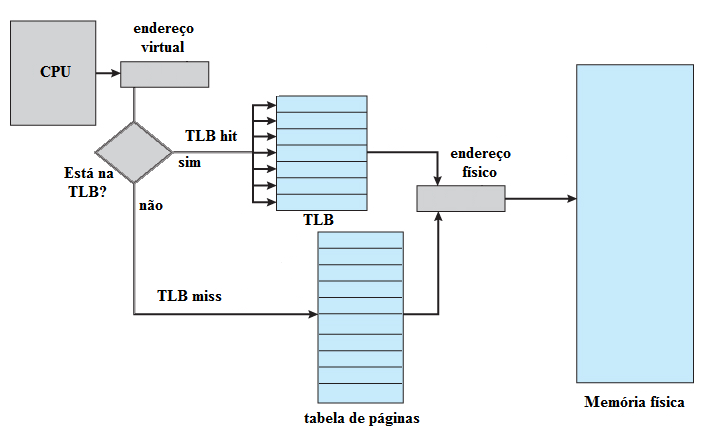
\includegraphics[scale=0.7]{figuras/tlbesquema.png}
\caption{Representação da arquitetura do processo de tradução}{Fonte: próprio autor}
\label{fig:arq}
\end{figure}

O fluxo desse funcionamento pode ser conferido na Figura \ref{fig:fluxo}. No processo de tradução de um endereço virtual, o sistema operacional verifica
primeiro a TLB. Se ocorrer uma TLB \textit{hit}, o processador acessa o endereço físico. Se ocorrer uma TLB \textit{miss}, será verificado se a página está na memória principal. Se sim, a tradução de seu endereço virtual é carregada na cache e o endereço é traduzido. Por outro lado, se não estiver na memória principal, o MMU faz uma chamada de sistema e indica
que houve falta de página. A página desejada precisa então ser carregada do disco para a
memória e se esta estive cheia, uma rotina de substituição de página é realizada. Em seguida, a tabela de páginas deve ser atualizada e os dados enviados para a TLB. Sempre
que há essa troca de contexto, a TLB deve ser reinicializada com as informações da nova
tabela de páginas. 
Tanto o processo de tratar falta de paginação quanto o de carregar na TLB as
informações novas, acabam sendo demorados, e influenciam no desempenho do sistema.

\begin{figure}[ht]
\centering
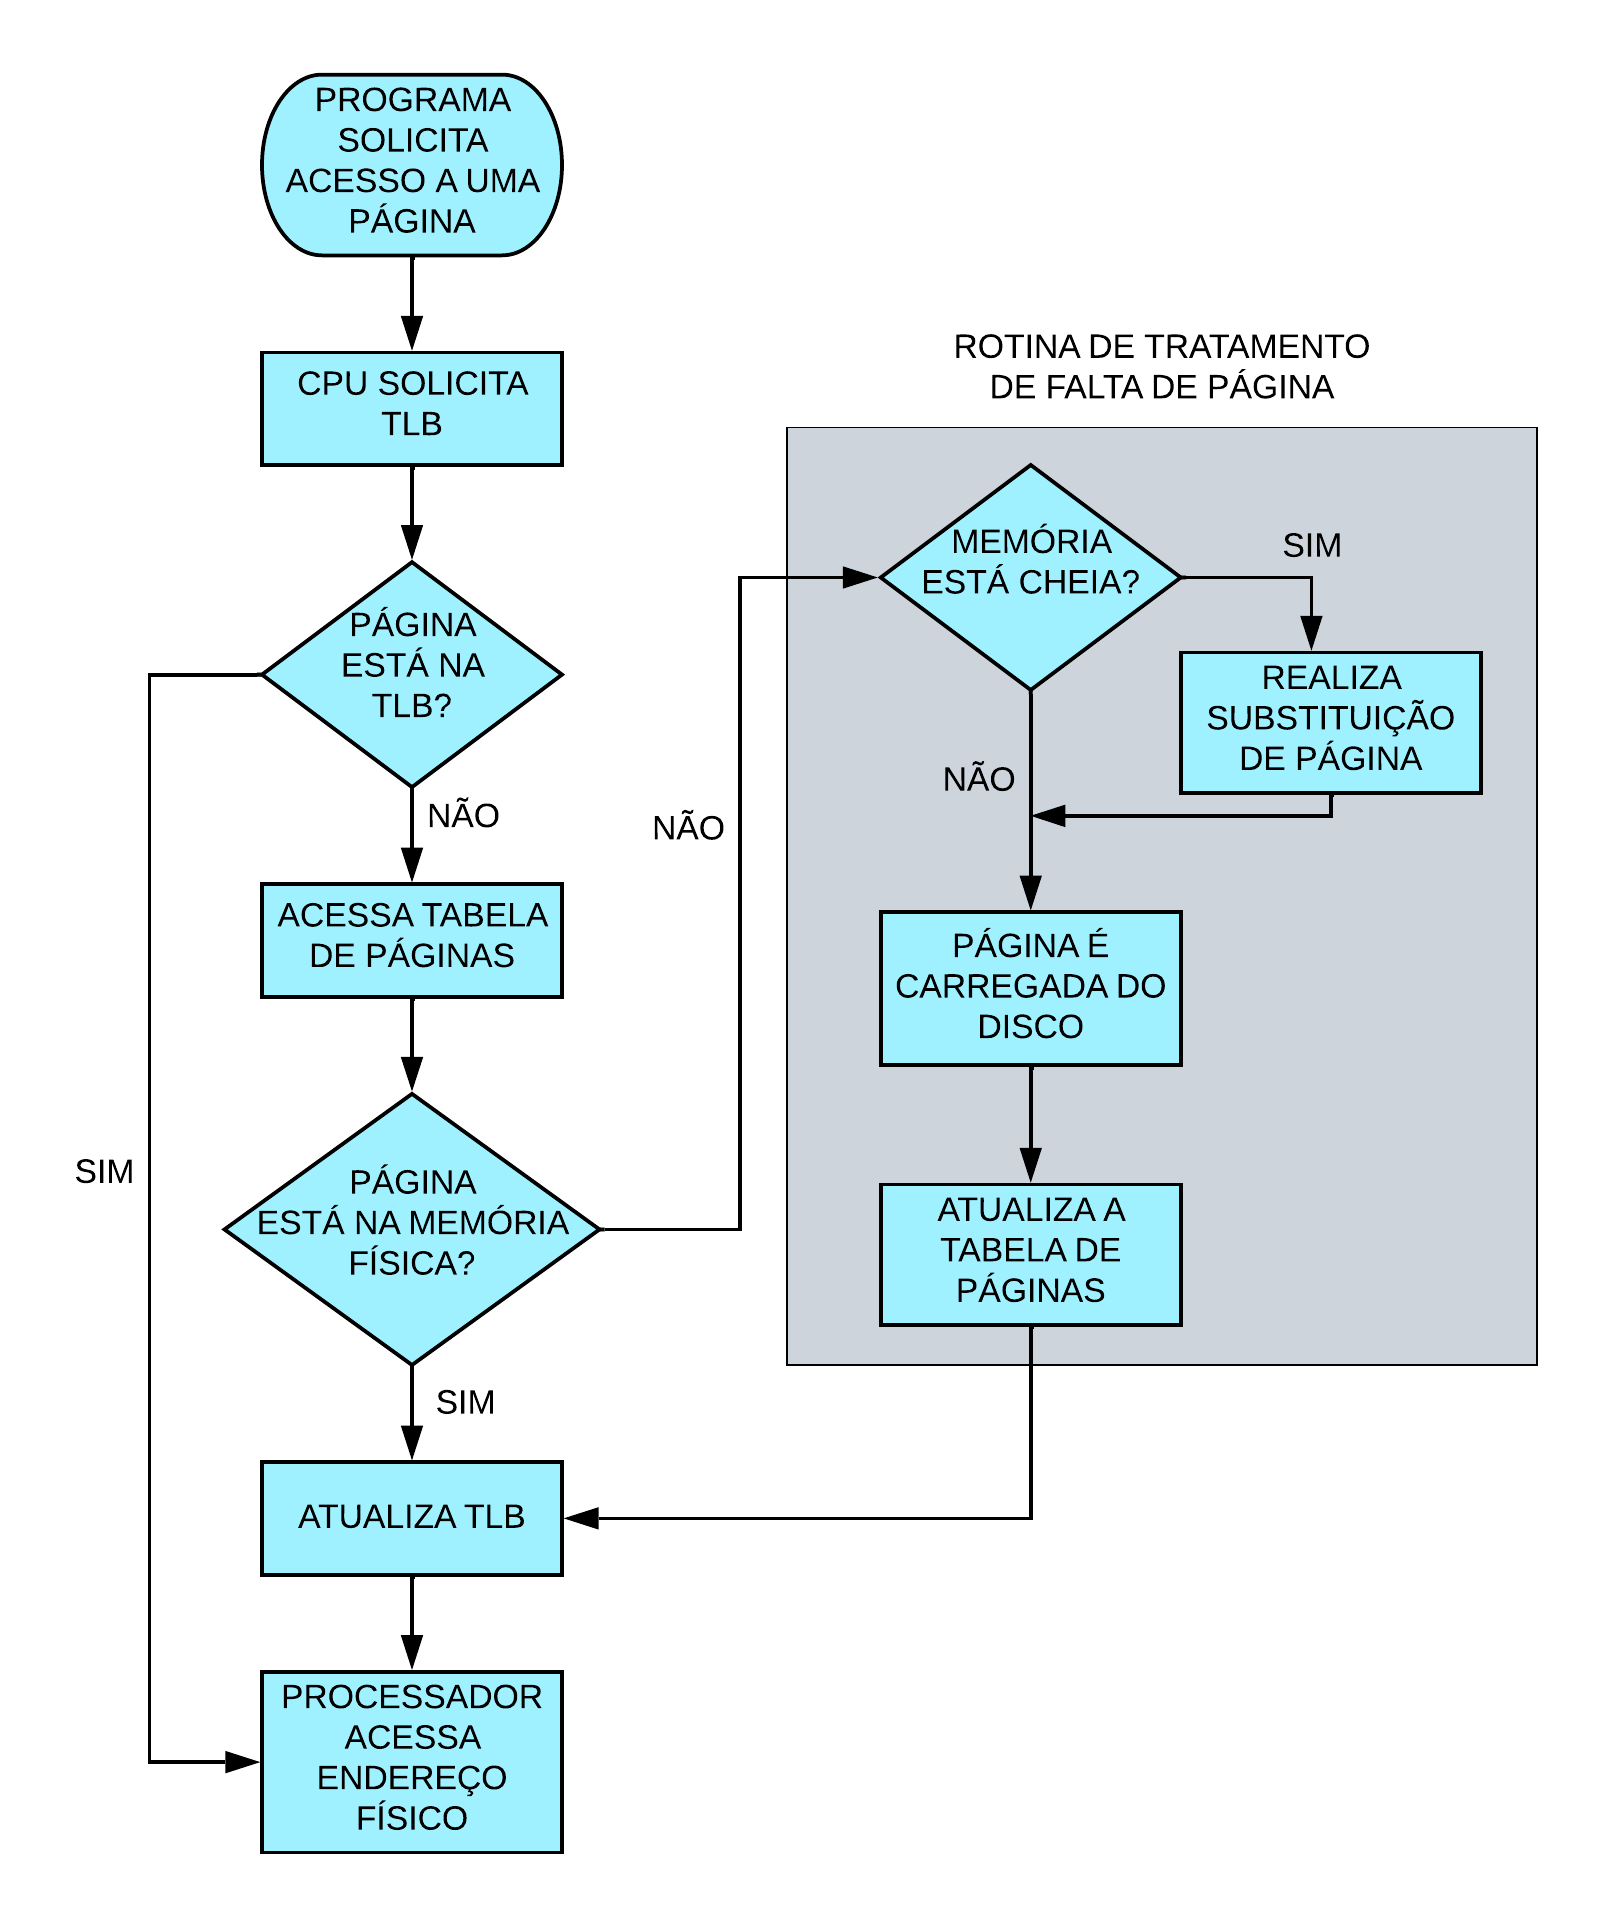
\includegraphics[scale=0.8]{figuras/fluxogramatlb.png}
\caption{Fluxograma do processo de tradução}{Fonte: próprio autor}
\label{fig:fluxo}
\end{figure}

\subsection{TLB \textit{miss} e TLB \textit{hit}}

A Figura \ref{fig:hit&miss} exemplificar melhor o que seria a TLB \textit{miss} e a TLB \textit{hit}, considerando um exemplo binário de endereço virtual com 8 bits: "11011001", que é buscado em uma TLB simples de 4 linhas. Nessa TLB estão os endereços "11011011", "11011010", "11011101", "11011000". São todos endereços próximos, mas nenhum igual ao requisitado. Acontece uma TLB \textit{miss} (a) e o processador busca o endereço na tabela de páginas. Se considerarmos que o endereço está na tabela de páginas, um algoritmo de substituição de páginas irá substituir um dos endereços que estavam na TLB anteriormente. No exemplo da figura, o endereço "11011011" foi substituído e a TLB foi atualizada com o endereço que estava sendo buscado. Se este mesmo endereço for buscado de novo, ele já está na TLB e acontece o \textit{hit} (b).

\begin{figure}[ht]
    \centering
      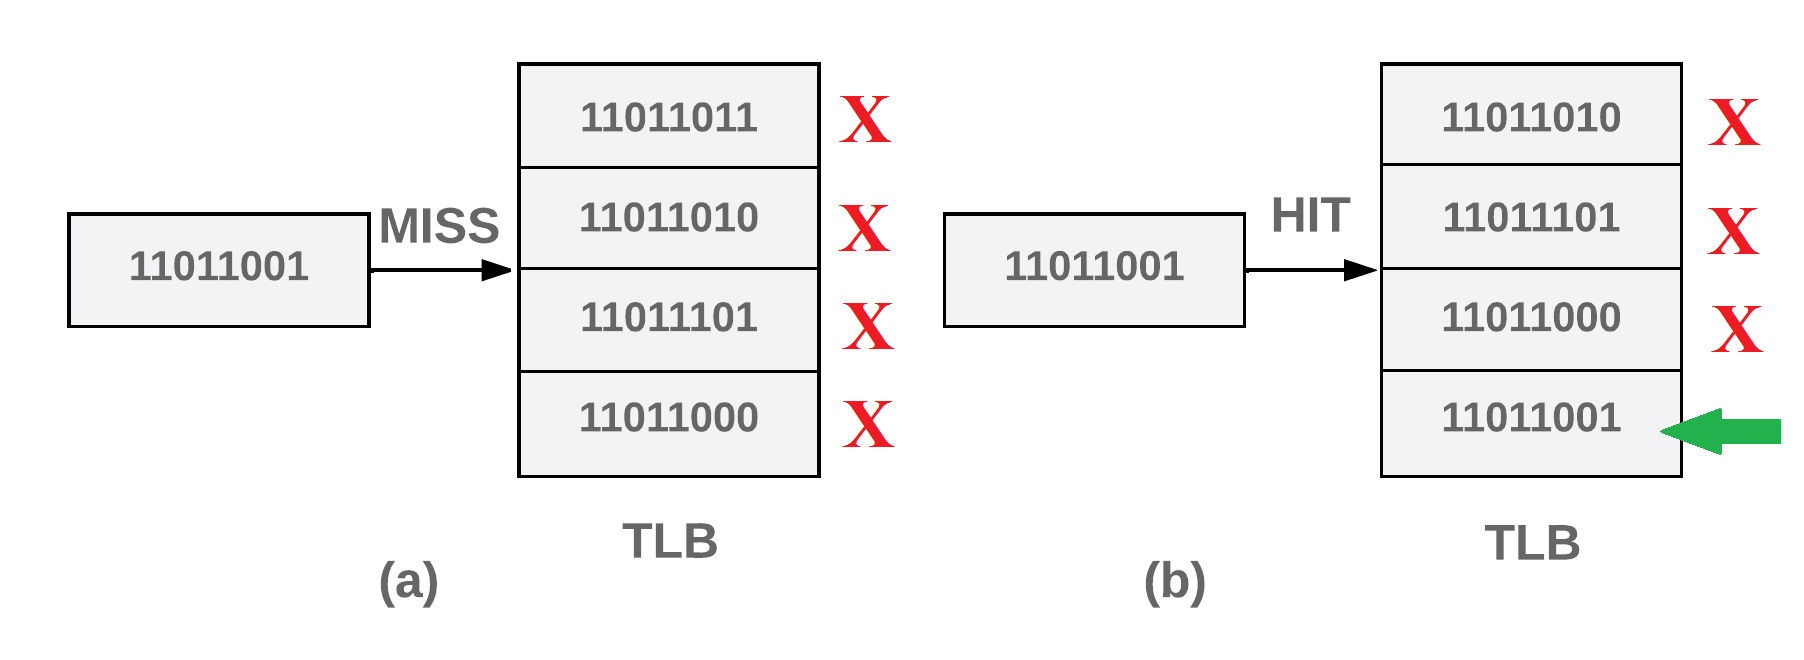
\includegraphics[scale=0.3]{figuras/hit&miss.png}
    \caption{Exemplo de TLB \textit{miss} (a) e TLB \textit{hit} (b)}{Fonte: próprio autor}
    \label{fig:hit&miss}
\end{figure}



\section{Falsos negativos e falsos positivos}

As entradas de uma TLB estão sujeitas a sofrerem com a ação de interferências externas, que podem alterar o valor do bit armazenado naquela célula de memória. Quando um erro atinge as entradas de uma TLB de instruções, podem ser produzidos dois tipos de falhas: falsos negativos e falsos positivos.

Falsos negativos acontecem quando os erros afetam os números das páginas
virtuais (NPVs) e o valor indicado pela TLB não corresponde mais ao valor original. Uma
falta de página é produzida e a nova informação deve ser recarregada da tabela de páginas da RAM. Na Figura \ref{fig:fneg}, inicialmente está representada uma TLB com alguns endereços de 8 bits (a). Em seguida, uma interferência atinge dois bits (b). Quando um um endereço é buscado pelo sistema, ele não coincide com os endereços na TLB (c). Neste caso, a TLB \textit{miss} resulta em uma rotina de tratamento de páginas e este processo pode atrapalhar o desempenho do sistema.

\begin{figure}[ht]
\centering
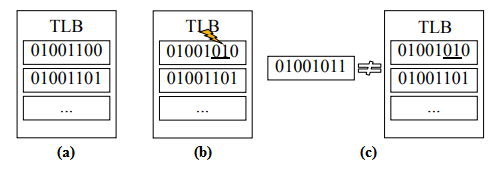
\includegraphics[scale=0.82]{figuras/FN_.PNG}
\caption{Falso negativo}{Fonte: próprio autor}
\label{fig:fneg}
\end{figure}

Por outro lado, no caso dos falsos positivos, o valor indicado pela TLB corresponde a uma página existente, no entanto, incorreta. Semelhante ao exemplo anterior, na Figura \ref{fig:fpos} tem-se a representação de um TLB (a), em que a falha também atinge dois bits (b). No entanto, dessa vez o endereço buscado coincide com o endereço após a alteração, gerando um falso positivo (c). Acontece um \textit{hit}, porém a tradução para endereço físico é errada. O número do endereço físico associado ao NPV é recuperado e uma instrução diferente da esperada é executada. Em casos extremos, isso pode causar falhas graves como congelamento do sistema ou até mesmo corrupção de dados. 

\begin{figure}[ht]
\centering
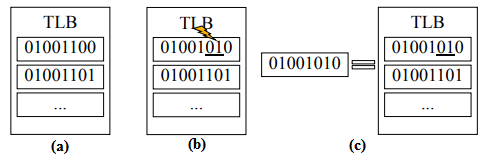
\includegraphics[scale=0.8]{figuras/FP_.PNG}
\caption{Falso positivo}{Fonte: próprio autor}
\label{fig:fpos}
\end{figure}

Considerando um exemplo semelhante ao visto na Figura \ref{fig:hit&miss} para melhor exemplificar estes conceitos, a Figura \ref{fig:fpex} representa um caso de falso positivo. Em (a) aconteceria um \textit{miss}, no entanto uma falha atinge o bit menos significativo do endereço "11011000", alternando seu valor para "11011001". Desse modo, em (b), a palavra buscada coincide com a que foi alterada. Como originalmente o endereço apontado era outro, a instrução errada vai ser executada.

\begin{figure}[ht]
    \centering
    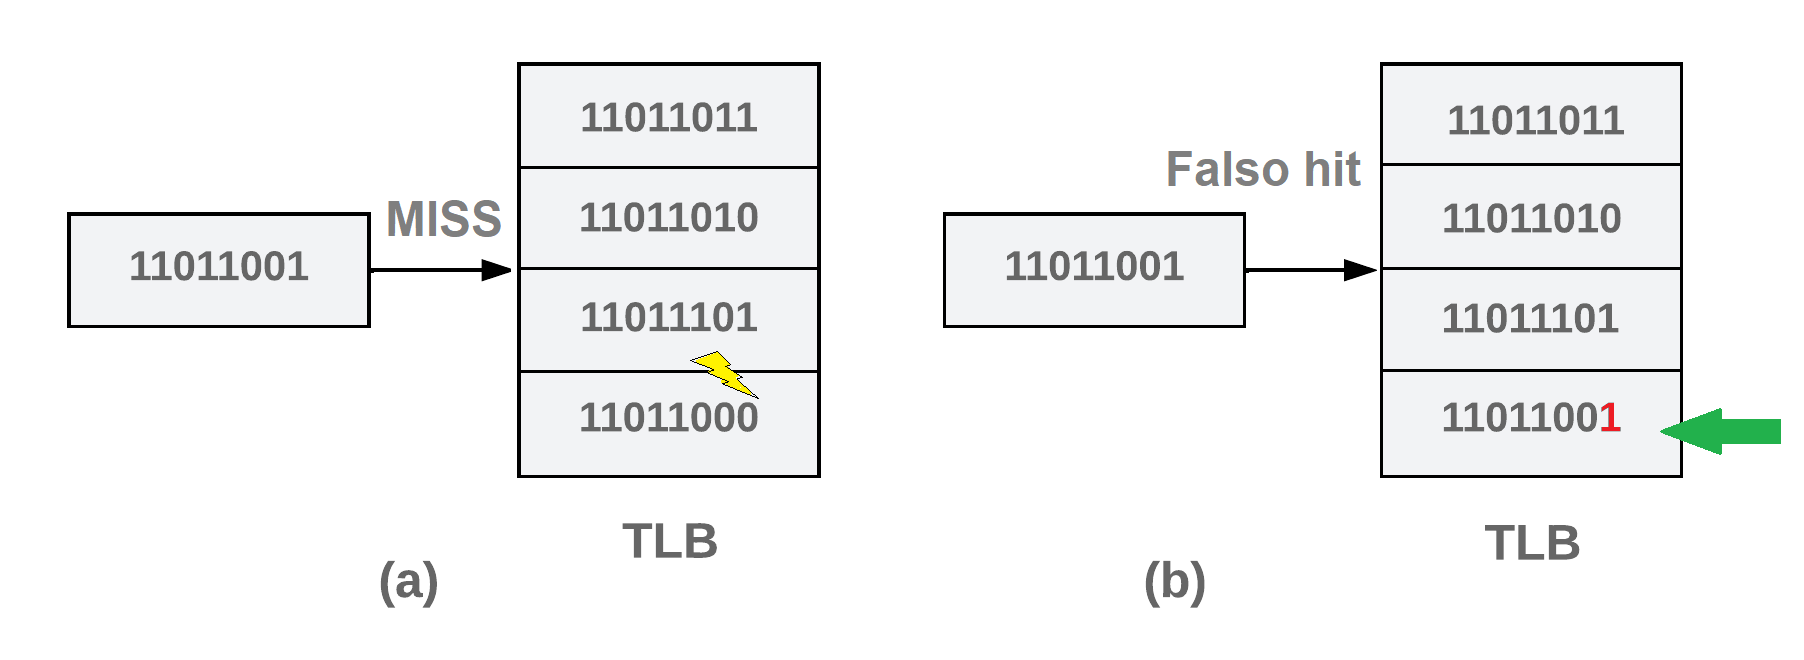
\includegraphics[scale=0.3]{modelo-dissertacao-ppgcc/figuras/FP.png}
    \caption{Exemplo de falso positivo}{Fonte:próprio autor}
    \label{fig:fpex}
\end{figure}

Do mesmo modo, a Figura \ref{fig:fnex} representa um exemplo de falso negativo. Considerando uma situação em que, em (a), haveria um \textit{hit}, já que existe coincidência entre a palavra buscada e um dos endereços da TLB. Se, nesse caso, uma falha atingisse o endereço "11011001" no "0" menos significativo, a palavra alterada seria "11011011". Assim, não há mais coincidência, logo a TLB indica uma \textit{miss}. O processo de tratamento de falta de página acontece sem necessidade, já que o endereço buscado já poderia ter sido apontado. Se recorrente, esse tipo de falha pode atrapalhar o desempenho do sistema.

\begin{figure}[ht]
    \centering
    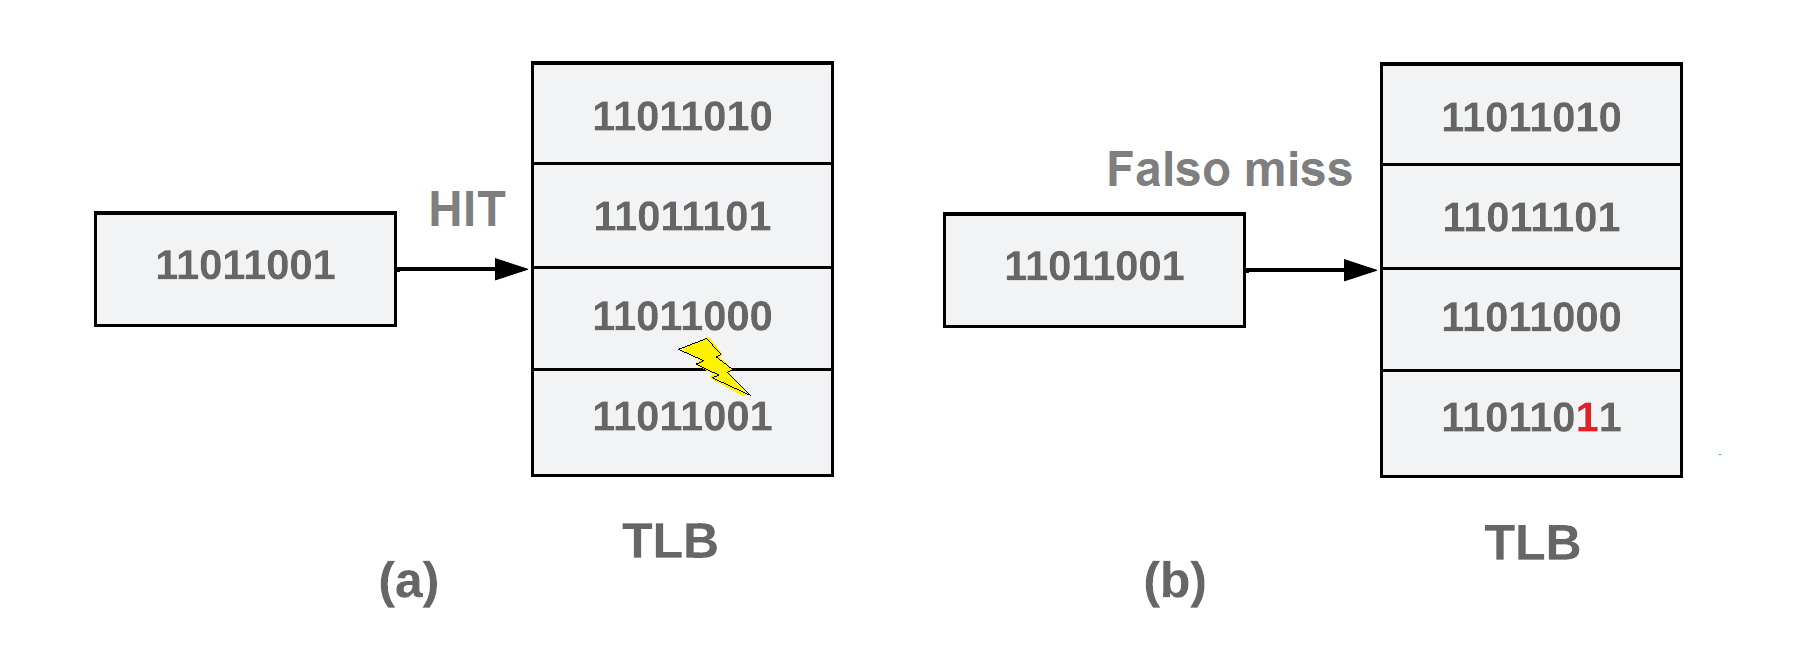
\includegraphics[scale=0.3]{modelo-dissertacao-ppgcc/figuras/FN.png}
    \caption{Exemplo de falso negativo}{Fonte:próprio autor}
    \label{fig:fnex}
\end{figure}

Os exemplos vistos mostram TLB pequenas e erros simples, mas essas falhas também acontecem em TLBs maiores e atingindo uma quantidade maior de bits. Os efeitos da radiação e outras interferências externas em circuitos cada vez mais integrados aumentam a possibilidade múltiplos bits atingidos.  

\section{A influência da radiação em dispositivos eletrônicos}

A radiação está presente em diversas formas e lugares, então dispositivos eletrônicos, mesmo em situações cotidianas, estão expostos a fatores que podem levá-los ao mau funcionamento. Em aplicações mais críticas, como as aplicações aeroespaciais, o sistema de memória está mais suscetível a interferências provenientes do ambiente, aumentando a ocorrência de MCUs \cite{varghese2013multiple}.

As junções de um transistor são muito sensíveis à radiação \cite{baumann2005soft}, então diversos eventos que acontecem à dispositivos orbitando a Terra podem alterar o estado de uma informação armazenada numa célula de memória ou durante uma transmissão de dados.

A figura a seguir mostra um exemplo de erro causado por interferências externas, apontando duas possíveis causas: uma queda de tensão ou causas ambientais como ondas eletromagnéticas \cite{vankeirsbilck2015integration}.

\begin{figure}[ht]
\centering
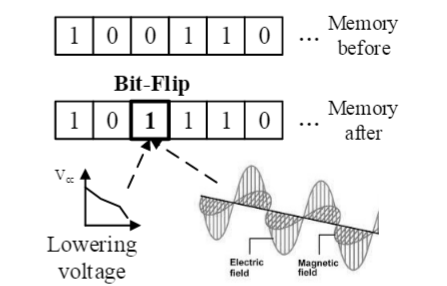
\includegraphics[scale=0.6]{figuras/error.PNG}
\caption{Exemplo de falha causada por interferências externas.}{Fonte: \cite{vankeirsbilck2015integration}}
\label{fig:error}
\end{figure}

\cite{slayman2005cache} disse que, em aplicações terrestres, a probabilidade de duas células de memória vizinhas serem afetadas por um erro durante um evento ionizante, é dez vezes menor que uma única célula. Enquanto \cite{seifert2008multi} mostraram que, em órbita, é muito mais provável a ocorrência de múltiplos erros. 

Os experimentos de \cite{satoh2000geometric} mostraram que as células afetadas são, na maioria das vezes, fisicamente próximas ou até mesmo adjacentes, após testes com sistemas de memória usando interferências externas espalhadas aleatoriamente pelas células. \cite{lawrence2008single} testaram sistemas de memórias para mostrar que single events upsets podem também afetar múltiplos bits, após ionização em diferentes aplicações.

Nesses cenários, códigos simples, como o cálculo de paridade e o código Hamming, não são o suficiente para minimizar os efeitos da radiação. Com isso, é necessário utilizar códigos mais robustos.

\section{Paridade}

Um dos métodos mais fáceis e mais utilizados para detecção de erros em sistemas de memória, é o cálculo da paridade. A codificação consiste em verificar a quantidade de bits em nível lógico alto e adicionar um bit com o valor da paridade. Normalmente as entradas de uma TLB já possuem um mecanismos de detecção de erros que utiliza o cálculo de um bit de paridade. Quando um erro é detectado, aquela entrada é invalidada e a TLB solicita novo envio \cite{griffith2005tlb}.

Existem dois tipos de paridade: 

\begin{itemize}
    \item paridade par: Quando um número binário (também chamado de palavra) possui um número par de 1's, então o bit de paridade será 0, para manter um número par de 1's. Desse modo, se o número de 1's é ímpar, então o bit de paridade será 1.
    \item paridade ímpar: Quando um número binário possui um número ímpar de 1's, então o bit de paridade será 0, para manter um número ímpar de 1's. Desse modo, se o número de 1's é par, então o bit de paridade será 1.
\end{itemize}

Para exemplificar isto, considerando a palavra 01100101, a quantidade de 1's nela é par. Neste caso, se a paridade for do tipo par, o bit de paridade será 0. Se a paridade for ímpar, então o bit de paridade será 1.

Essa operação pode ser representada por $\oplus$, que simboliza a porta lógica Ou-Exclusivo, ou apenas XOR. No caso do exemplo acima, utilizando paridade par, temos:
\begin{equation}
    0 \oplus 1 \oplus 1 \oplus 0 \oplus 0 \oplus 1 \oplus 0 \oplus 1 = 0
\end{equation}

Desse modo, o bit adicionado à palavra é 0, então a palavra codificada é 001100101, onde o 0 mais à esquerda é o bit de paridade (BP).
Se uma falha atinge uma célula de memória e um dos bits de nível lógico baixo muda seu valor de 0 para 1 (indicado abaixo em negrito), a nova quantidade de 1's agora é ímpar e o bit de paridade adicionado deveria ser 1.
\begin{equation}
    \textbf{1} \oplus 1 \oplus 1 \oplus 0 \oplus 0 \oplus 1 \oplus 0 \oplus 1 = 1
\end{equation}
    
O processador codifica a palavra como 111100101, sendo o 1 mais à esquerda o novo bit de paridade(BP'). A detecção de erro ocorre quando os dois bits de paridade são comparados.
\begin{equation}
    BP \oplus BP' = 0 \oplus 1 = 1
\end{equation}

Assim, é indicada a presença de erro na palavra armazenada.

Deste ponto em diante, sempre que for citado paridade neste trabalho, estará sendo considerada a paridade par.


\section{Código Hamming}

O matemático americano Richard Hamming criou em 1950 um código de detecção e correção que recebeu seu nome \cite{milies2009breve}. Até hoje, o código Hamming é bastante utilizado em diversas aplicações na computação, inclusive como base para outros códigos de correção de erro. O código permite não só detectar a presença de um erro, mas também a sua localização. Sabendo a posição do bit alterado na palavra, é possível corrigi-lo. Além disso, consegue detectar até dois bits com erros. Portanto, o Hamming é um código do tipo SEC-DED (Single Error Correction - Double Error Detection).

Como pode ser visto na Figura \ref{fig:hamming}, o código Hamming ocorre da seguinte maneira: os bits de redundância são adicionados intercalados aos bits da palavra original (a), e seus valores são calculados de uma forma específica (b). Por exemplo, o bit de paridade P1 é o resultado de D1 $\oplus$ D2 $\oplus$ D4.

\begin{figure}[ht]
    \centering
    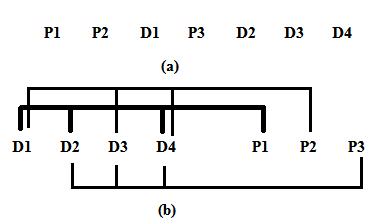
\includegraphics[scale=0.7]{figuras/hamming.png}
    \caption{Código Hamming, distribuição dos bits (a) e cálculo de paridades (b)}{Fonte: próprio autor}
    \label{fig:hamming}
\end{figure}

O número de bits de redundância depende do número de bits de dados, seguindo a equação 
\begin{equation}
    2^m-1=n
\end{equation}
em que m é o número de bits de redundância e n o número total de bits da palavra codificada.


\section{Trabalhos Relacionados}

A teoria moderna de códigos originou-se com o trabalho de Claude Shannon, que teve papel importante na base teórica do que hoje chamamos códigos corretores de erros \cite{meneghesso2012codigos}. A ideia central desses códigos usados em sistemas de memória é a adição de bits de redundância nos dados a serem transmitidos, codificando-os. Os receptores usam essas redundâncias para verificar a consistência da mensagem, podendo,
caso encontre erro, corrigi-lo por meio da decodificação.

Alguns dos códigos corretores de erros mais antigos são os da família Reed-Muller, desenvolvidos na década de 1950 e sendo utilizado em aplicações espaciais. Foi implementado nas sondas Mariner, que transmitiam fotos da superfície de Marte \cite{varghese2013multiple}.

Outro desses códigos capazes de lidar com MCUs em memórias é o código Matrix \cite{argyrides2007matrix}. Esse código associa o código de Hamming com paridade, codificando uma palavra em formato matricial. O Reed-Muller é mais robusto que o Matrix e apresenta taxa de correção maior, no entanto, os custos de implementação do Matrix são muito menores.

Outras formas de codificar palavras binárias vêm sendo propostas e estudadas nos últimos anos. A seguir serão apresentadas algumas delas.

\subsection{Códigos de correção de erros}

Usando conceitos de Hamming Estendido e paridade, o \textit{Column Line Code} (CLC) \cite{castro2016correction} é um código matricial que apresenta custo de implementação bem mais baixos que o Reed-Muller e taxas de correção maiores que o Matrix. A Figura \ref{fig:clc} mostra como se distribui os bits de redundância adicionados após a codificação do CLC. Na figura, C são os bits de dados, CB são calculados a partir do Hamming de cada linha de dados, Pa é o resultado do Hamming Estendido, e P são as paridades, calculadas para cada coluna. Posteriormente, \cite{silva2018extensible} apresenta uma versão melhorada do CLC, o CLC Estendido, que incrementa as capacidades de proteção do código.

\begin{figure}[ht]
    \centering
    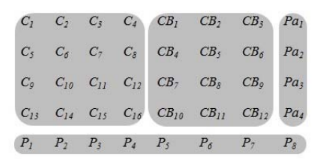
\includegraphics[scale=1]{figuras/clc.PNG}
    \caption{Codificação do CLC com 16 bits de entrada}{Fonte: \cite{castro2016correction}}
    \label{fig:clc}
\end{figure}

Numa nova melhoria do código, os autores  apresentam, o CLC-A, que fica alternando entre o CLC Padrão e o CLC Estendido de acordo com o tipo de erro detectado, e essa alternância interfere positivamente nos resultados \cite{silva2020clc}. O método funciona muito bem para corrigir múltiplos erros, mas o trabalho mais recente não faz uma comparação com outras abordagens, apenas com as versões anteriores. No entanto, o problema desse código é que acrescenta muitos bits de redundância, demandando muito poder computacional.

O \textit{Parity Hamming Interleaved Correction Code} (PHICC) é um dos códigos matriciais mais recentes, desenvolvido para ser um código de baixo custo computacional além de possuir uma grande capacidade de correção de erros, unindo paridade, Hamming e intercalação \cite{magalhaes2019phicc}.

A Figura \ref{fig:phicc} demonstra como fica a palavra após o processo de codificação dos bits de entrada com um exemplo de 16 bits. O objetivo da intercalação é redistribuir possíveis aglomerados de erros, de modo a facilitar a detecção dos mesmos. Na figura, C são os bits de entrada já intercalados, Ppl e Ppc representam respectivamente a paridade dessas linhas e colunas, CB são os resultados da codificação Hamming para cada linha de dados antes de intercala e, por fim, Dp é simplesmente a paridade das linhas de dados também antes de intercalar. 

\begin{figure}[ht]
    \centering
    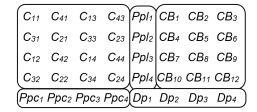
\includegraphics[scale=1]{figuras/phicc.PNG}
    \caption{Codificação do PHICC com 16 bits de entrada}{Fonte: \cite{magalhaes2019phicc}}
    \label{fig:phicc}
\end{figure}

Apesar de conseguir reduzir o custo da implementação, esse modelo acrescenta muitos bits e possui uma lógica de codificação complicada, podendo sobrecarregar a memória.      

\subsection{Técnicas de proteção para a CAM e TLB}

A abordagem de \cite{pagiamtzis2006soft} se utilizou da adição de um bit de paridade nos endereços para aumentar a distância Hamming entre endereços próximos. Este método servia para detectar bits com erros. Além disso, para melhorar a proteção contra erros, o esquema as técnicas de verificação do \textit{match line}. O método reduz a quantidade de erros nas células de memória sem acrescentar tempo de execução, mas adiciona área devido aos bits extras. A Figura \ref{fig:matchline} é uma representação desse esquema, onde pode ser vista a área adicionada referente à paridade. As células com D representam os bits armazenados e com P são os resultados das paridades de cada linha.

\begin{figure}[ht]
    \centering
    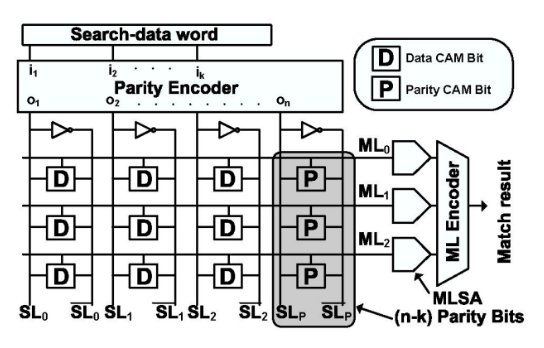
\includegraphics[scale = 0.7]{figuras/matchline.png}
    \caption{Esquema de proteção de CAM com paridade e aprimoramento do matchline}{Fonte: \cite{pagiamtzis2006soft}}
    \label{fig:matchline}
\end{figure}

Técnicas de redundância espacial foram utilizadas por \cite{lang2013processor} e \cite{maestro2013soft} para minimizar falhas nas células de memória. O primeiro usava uma cópia de \textit{back-up} com o conteúdo da TLB. Quando um erro era detectado, a TLB era simplesmente sobrescrita com a cópia. Já em \cite{maestro2013soft}, a técnica de duplicação era acompanhada por algoritmos capazes de detectar uma quantidade maior de erros, o que diminuía as falhas. Apesar disso, as duas técnicas duplicam o espaço de memória necessário para implementação.

Em \cite{sanchez2016combined}, os autores usam Hamming e paridade para implementar um código matricial SEC-DAED (do inglês, \textit{single error correction - double adjacent error detection}) que proteja CAMs e memórias associativas, como as TLBs. Protegendo sistemas de memória em geral, \cite{sanchez2012hamming} através da utilização de Hamming Estendido, implementa um código do tipo SEC-DED-TAED (do inglês, \textit{single error correction - double error detection - triple adjacent error detection}).

\cite{li2018efficient} propõe um código linear para tratar erros em TLBs, utilizando intercalação para codificar a palavra. O método se trata de dividir a palavra recebido em 4 grupos de bits e realizar cálculos de paridade entre esses grupos. Devido ao processo de intercalação, o código consegue tratar erros simples e duplo adjacentes. Além disso, no mesmo trabalho, os autores apresentam uma abordagem para minimizar a quantidade de bits de redundância em códigos para corrigir até erros quádruplos. Na Figura \ref{fig:4bit} está representada a lógica do circuito deste método, onde são avaliados diversos cenários com possibilidades de falhas em até 4bits. Na figura, cada "X" representa um bit com erro e "C" um bit correto. Por exemplo, XCXX possui uma configuração com um erro triplo, sendo que dois bits com erro são adjacentes. Comparado com outros métodos lineares, este acaba acrescentando ocupando muita área na implementação. 

\begin{figure}[ht]
    \centering
    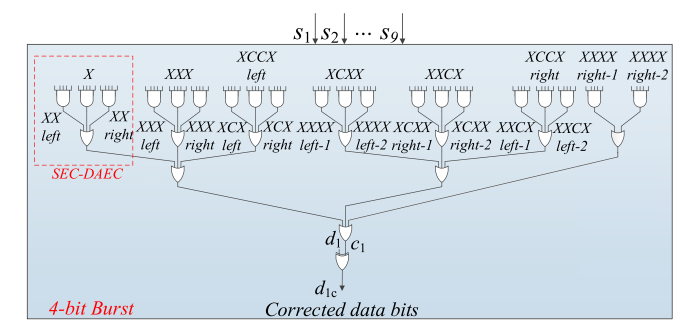
\includegraphics[scale=0.7]{modelo-dissertacao-ppgcc/figuras/4bitburst.PNG}
    \caption{Decodificação do código para  grupos de 4-bit de erros}{Fonte: \cite{li2018efficient}}
    \label{fig:4bit}
\end{figure}

Os autores de  \cite{kiani2019improving} apresentam um código em formato matricial com o objetivo de proteger TLBs contra falsos positivos. O esquema proposto também utiliza paridade para detectar e corrigir erros.  Na avaliação do código, foram analisados dois cenários: o primeiro reduz a capacidade de armazenamento da TLB para usar esse espaço para armazenar os bits de paridade, enquanto o segundo adiciona linhas e/ou colunas extras para fazer esta alocação. As taxas de correção são boas para erros simples e duplos, mas falham para erros triplos.

Uma abordagem focada na proteção de TLBs é apresentada em \cite{sanchez2019reducing}. Esse método será utilizado nos experimentos realizados neste trabalho, portanto ele será mais detalhado em uma seção própria, a seguir. 

\section{Paridade codificada nos NPVs}

O trabalho de \cite{sanchez2019reducing} propõe um método utilizado para diminuir a ocorrência de falsos positivos nas TLBs, aproveitando do conhecimento do princípio de localidade (ou localidade de referência). Sua abordagem trata da codificação dos números que representam as páginas virtuais (NPVs) de uma maneira específica antes que estes sejam armazenados nas TLBs. O método em questão foi implementado em um\textit{ Field Programmable Gate Array} (FPGA) e comparado com um esquema anterior, mostrando que ele pode fornecer melhor proteção para endereços vizinhos, sem custo adicional. A abordagem funciona bem, corrigindo até erros triplos adjacentes. 

Como pode ser visto na Figura \ref{fig:codeS}, o NPV é codificado e apresentado à TLB com a nova configuração. Neste método, não é necessário decodificar NPV’. Quando a CPU solicita um NPV, ele é codificado e a TLB tenta combiná-lo com os valores armazenados na CAM. Se houver o hit, o endereço físico será retornado. Se houver o miss, uma falha de página é emitida

\begin{figure}[ht]
    \centering
    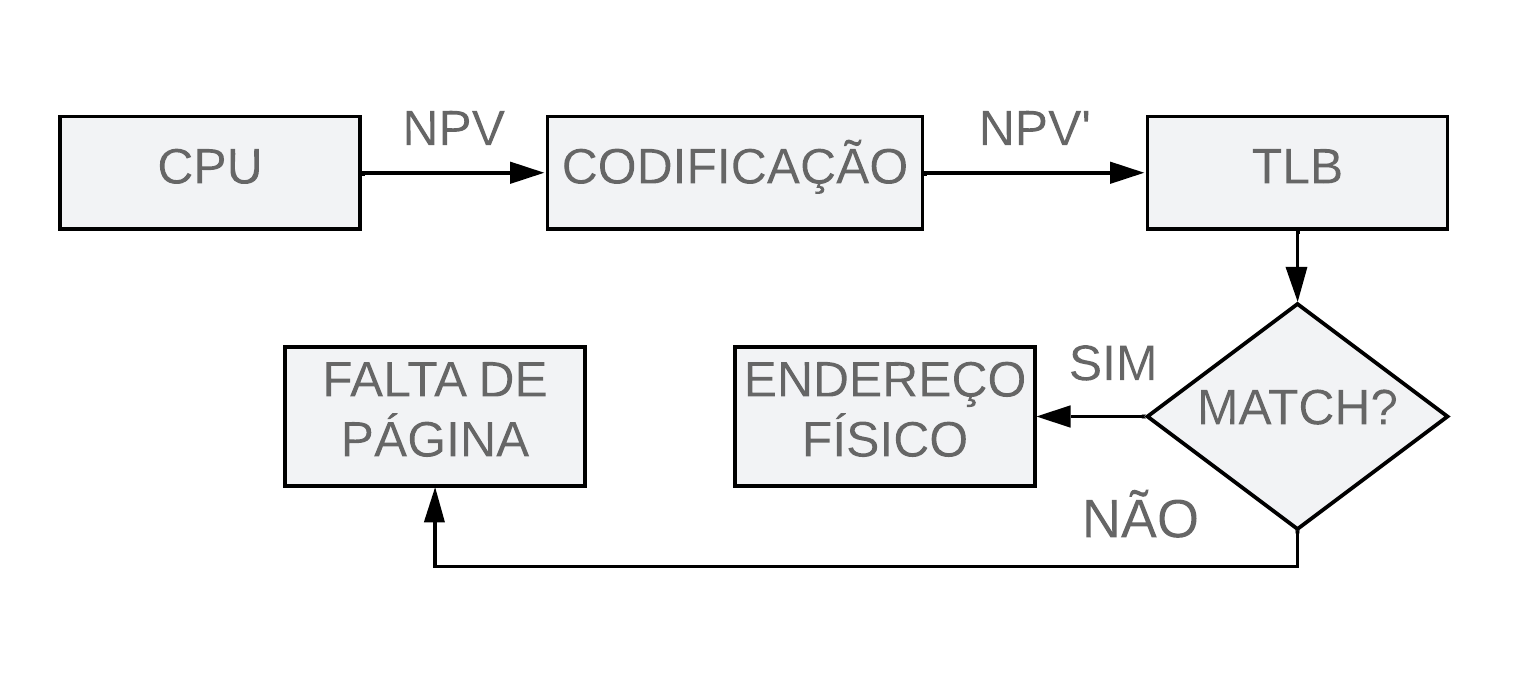
\includegraphics[scale=0.9]{figuras/match.png}
    \caption{Codificação e verificação de \textit{match}}{Fonte: próprio autor}
    \label{fig:codeS}
\end{figure}

A proposta do trabalho de \cite{sanchez2019reducing} era codificar os dois bits mais significativos (MSB, do inglês \textit{most significant bit}) de modo que sobrescrevesse nesses bits o resultado da paridade dos bits do NPV na TLB, alternando entre posições pares e ímpares, como mostrado a seguir.
\begin{equation}
    NPV'[MSB] = NPV[MSB] \oplus NPV[MSB-2] \oplus ... NPV[1]
\end{equation}
\begin{equation}
    NPV'[MSB-1] = NPV[MSB-1] \oplus NPV[MSB-3] \oplus ... NPV[0]
\end{equation}    
    

Os demais bits que não são os MSB ou o MSB-1 permanecem inalterados após a codificação. Na implementação física do esquema descrito, no cenário com um NPV de 32 bits, o circuito fica semelhante ao da Figura \ref{fig:32}. Uma porta XOR simples realiza a operação de paridade entre duas entradas, cada entrada desta representando um bit do NPV. Deste modo, são necessárias 30 portas XOR para chegar aos resultados das paridades que sobrescreverão os valores de MSB e MSB-1.

\begin{figure}[ht]
\centering
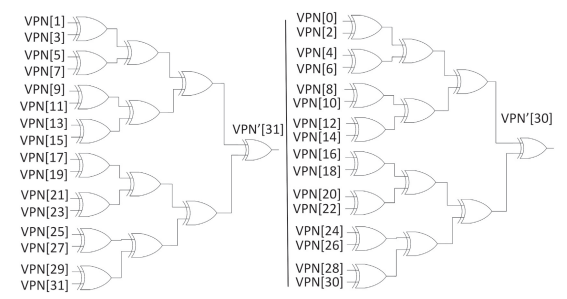
\includegraphics[scale=0.7]{figuras/32bit.png}
\caption{Circuito com as portas xor do cenário com 32 bits}{Fonte: \cite{sanchez2019reducing}}
\label{fig:32}
\end{figure}

Utilizando um exemplo de palavra com oito bits para simplificar a explicação: considere o NPV igual a 10100011. O bit mais significativo (MSB) é o bit 1 mais à esquerda, assim como o segundo bit mais significativo (MSB-1) é bit 0 à direita do MSB.

As equações para calcular o MSB e o MSB-1 a substituir os atuais ficam: 
\begin{equation}
   NPV'[MSB] = 1 \oplus 1 \oplus 0 \oplus 1    
\end{equation}
\begin{equation}
    NPV'[MSB-1] = 0 \oplus 0 \oplus 0 \oplus 1
\end{equation}
Nesse caso, o valor do MSB permanece 1, já que existe um número ímpar de bits 1, enquanto o MSB-1, pelo mesmo motivo, é convertido de 0 para 1. A nova palavra, o VPN', que será armazenada na TLB na mesma posição é 11100011.

A codificação por paridade nos NPVs incrementa a distância Hamming entre endereços vizinhos em dois bits. Isto garante que se as células de memória da TLB forem afetadas por um erro em um bit, nenhum \textit{single erorr} será produzido. Do mesmo modo, \textit{double adjacent errors} também são evitados, devido ao processo de calcular bits pares e ímpares separadamente.

\section{Conclusão}

A Tabela 1, a seguir, é um quadro comparativo com um resumo dos trabalhos relacionados citados anteriormente, apontando características da publicação e quais foram as abordagens e técnicas de codificação utilizadas em cada um. Percebe-se que paridade e Hamming são as técnicas de codificação mais utilizadas.

\begin{table}[ht]
\footnotesize
\centering
\caption{Quadro comparativo com resumo dos trabalhos relacionados}
\begin{tabular}{
>{\columncolor[HTML]{EFEFEF}}l |l|l|l}
\hline
\multicolumn{1}{c|}{\cellcolor[HTML]{EFEFEF}\textbf{\begin{tabular}[c]{@{}c@{}}Nome do\\ artigo\end{tabular}}} & \multicolumn{1}{c|}{\cellcolor[HTML]{EFEFEF}\textbf{\begin{tabular}[c]{@{}c@{}}Autores e ano de\\ publicação\end{tabular}}} & \multicolumn{1}{c|}{\cellcolor[HTML]{EFEFEF}\textbf{Abordagem}} & \multicolumn{1}{c}{\cellcolor[HTML]{EFEFEF}\textbf{\begin{tabular}[c]{@{}c@{}}Técnicas de\\ codificação\end{tabular}}} \\ \hline
\begin{tabular}[c]{@{}l@{}}CLC-A: An adaptive\\ implementation\\ of the Column\\ Line Code (CLC)\\ ECC\end{tabular} & \begin{tabular}[c]{@{}l@{}}Silva, Felipe et al.,\\ 2020\end{tabular} & Matricial. & \begin{tabular}[c]{@{}l@{}}Hamming Estendido e\\ paridade. Aprimora o\\ CLC padrão e o CLC\\ estendido\end{tabular} \\ \hline
\begin{tabular}[c]{@{}l@{}}PHICC: An error\\ correction code for\\ memory devices\end{tabular} & \begin{tabular}[c]{@{}l@{}}Magalhães et al.,\\ 2019\end{tabular} & Matricial. & \begin{tabular}[c]{@{}l@{}}Paridade, Hamming\\ e intercalação\end{tabular} \\ \hline
\begin{tabular}[c]{@{}l@{}}Reducing false\\ positives due to \\ double adjacent \\ errors in\\ instruction TLBs\end{tabular} & \begin{tabular}[c]{@{}l@{}}Sanchez-Mácian\\ et al., 2019\end{tabular} & \begin{tabular}[c]{@{}l@{}}Linear. Distancia\\ Hamming\end{tabular} & \begin{tabular}[c]{@{}l@{}}Paridade entre os bits,\\ alternando entre par e\\ ímpar, para armazenas\\ nos 2 MSBs\end{tabular} \\ \hline
\begin{tabular}[c]{@{}l@{}}Improving instruction\\ TLB reliability with\\ efficient multi-bit \\ soft error protection\end{tabular} & \begin{tabular}[c]{@{}l@{}}Kiani e Reviriego,\\ 2019\end{tabular} & Matricial. & \begin{tabular}[c]{@{}l@{}}Paridade vertical e\\ horizontal, alternando\\ entre par e ímpar. Uso\\ do espaço da TLB para\\ paridades\end{tabular} \\ \hline
\begin{tabular}[c]{@{}l@{}}Efficient\\ implementations of\\ 4-bit burst error\\ correction for\\ memories\end{tabular} & Li et al., 2018 & Linear & Intercalação e paridade \\ \hline
\begin{tabular}[c]{@{}l@{}}Combined modular\\ key and data error\\ protection for\\ content-addressable\\ memories\end{tabular} & \begin{tabular}[c]{@{}l@{}}Sanchez-Mácian,\\ Reviriego e\\ Maestro, 2016\end{tabular} & SEC-DAED & Hamming e paridade \\ \hline
\begin{tabular}[c]{@{}l@{}}Soft error tolerant\\ content-addressable\\ memories (cams)\\ using error detection\\ codes and duplication\end{tabular} & Maestro, 2013 & \begin{tabular}[c]{@{}l@{}}Redundância\\ espacial\end{tabular} & \begin{tabular}[c]{@{}l@{}}Duplicação da TLB e\\ algoritmo de detecção\end{tabular} \\ \hline
\begin{tabular}[c]{@{}l@{}}Processor fault \\ tolerance, through\\ translation lookaside\\ buffer refresh\end{tabular} & Lang, 2013 & \begin{tabular}[c]{@{}l@{}}Redundância\\ espacial\end{tabular} & \begin{tabular}[c]{@{}l@{}}Cópia da TLB e\\ atualização ao\\ encontrar erro\end{tabular} \\ \hline
\begin{tabular}[c]{@{}l@{}}A Hamming sec-daed\\ and extended\\ hamming sec-ded-taed\\ codes thtough\\ selective shortenning\\ and bit placement\end{tabular} & \begin{tabular}[c]{@{}l@{}}Sanchez-Mácian,\\ Reviriego e\\ Maestro, 2012\end{tabular} & \begin{tabular}[c]{@{}l@{}}SEC-DED-\\ TAED\end{tabular} & \begin{tabular}[c]{@{}l@{}}Hamming estendido\\ e paridade\end{tabular} \\ \hline
\begin{tabular}[c]{@{}l@{}}A soft-error toletant\\ content-addressable\\ memory (cam) using\\ an error-correction-\\ match-scheme\end{tabular} & \begin{tabular}[c]{@{}l@{}}Pagiamtzis, Azizi\\ e Najm, 2016\end{tabular} & \begin{tabular}[c]{@{}l@{}}Distancia \\ Hamming\end{tabular} & \begin{tabular}[c]{@{}l@{}}Aprimoramento do\\ match-line da CAM\end{tabular} \\ \hline
\end{tabular}
\end{table}

Com os conceitos apresentados neste capítulo, é possível entender com mais facilidade a proposta dessa pesquisa. O método exposto na seção 2.9 será explorado neste trabalho em outra abordagem, afim de obter resultados com menor custo de implementação. No próximo capítulo, serão mostrados a metodologia deste trabalho e detalhes dos experimentos realizados.

 			% Capitulo de exemplo
\chapter{Metodologia}
\label{cap:4}

Este capítulo apresenta as etapas de desenvolvimento deste trabalho, além de mostrar os códigos propostos e a descrição dos experimentos realizados.

\section{Desenvolvimento do Trabalho}

A metodologia deste trabalho adotou o passo-a-passo exposto na Figura \ref{fig:metodologia}. Inicialmente, foi feita uma pesquisa bibliográfica sobre os temas relacionados a códigos de correção de erros, proteção de TLBs e o efeito da radiação em dispositivos eletrônicos. Realizadas as principais leituras, começamos a desenvolver o código do simulador de TLB, na linguagem de programação Python. O simulador de TLB implementado apresenta as seguintes configurações: cache totalmente associativa, com 8 posições de memória e algoritmo de substituição LRU (do inglês, \textit{least recently used}), além de um NPV com 32 bits.

\begin{figure}[ht]
    \centering
    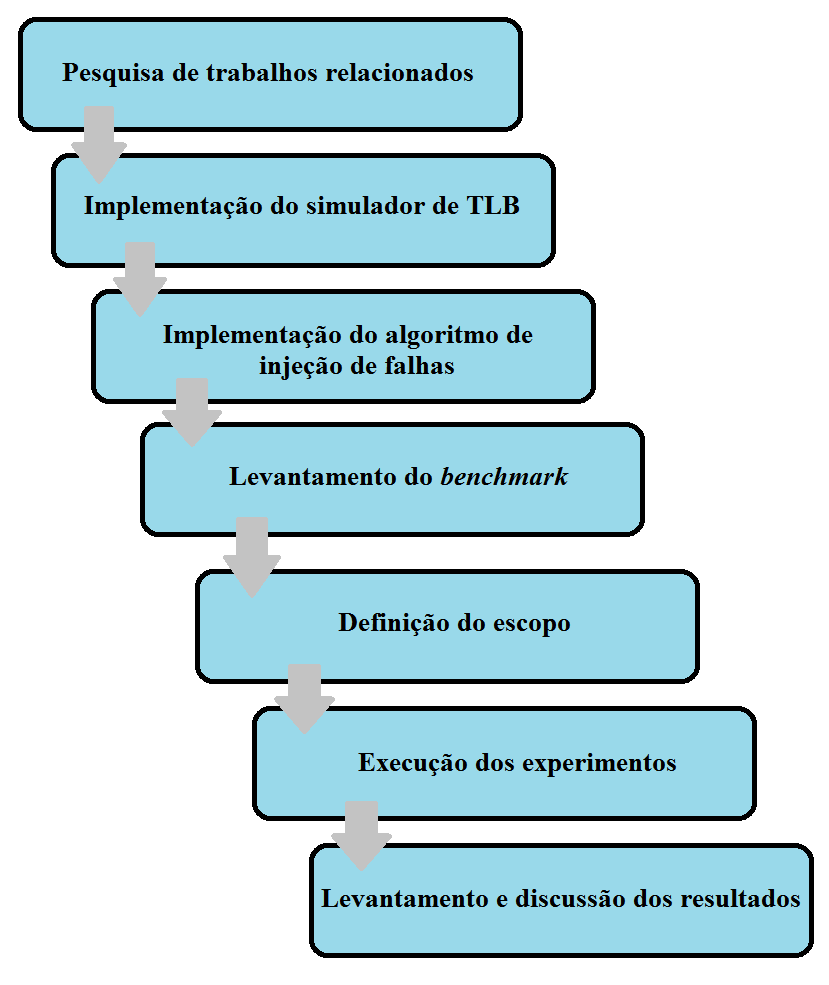
\includegraphics[scale=0.42]{figuras/metodologia.png}
    \caption{Fases do desenvolvimento do trabalho}{Fonte: próprio autor}
    \label{fig:metodologia}
\end{figure}

Em seguida, foi feita a implementação da injeção de falhas. O algoritmo de injeção de falhas desenvolvido é pseudo-aleatório, ocorrendo em posições diferentes a cada nova execução, de acordo com três parâmetros: endereço de falha, que diz em que momento da execução a falha será inserida; linha da tlb, que diz em qual das 8 posições da TLB a falha será injetada; e bit falho, que é referente a qual a posição da falha no NPV, existindo 32 possibilidades de posição. Injetar uma falha em um bit, tendo todos os parâmetros já sorteados, trata-se de alterar o valor desse bit, de 0 para 1 ou vice-versa. Se o tipo de falha é dupla, vai atingir o bit sorteado e o vizinho da direita. Se é falha tripla, atinge os dois vizinhos. A Figura \ref{fig:falhas} apresenta um exemplo para cada um dos três tipos de falha: falha simples (a) atingindo um único bit, falha dupla adjacente atingindo o vizinho da direita (b), e falha tripla adjacente atingindo ambos os vizinhos (c).

\begin{figure}[ht]
    \centering
    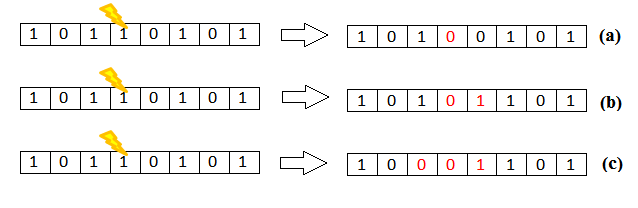
\includegraphics[scale=0.8]{modelo-dissertacao-ppgcc/figuras/falhas.PNG}
    \caption{Exemplos de falha simples (a), falha dupla (b) e falha tripla (c)}{Fonte: próprio autor}
    \label{fig:falhas}
\end{figure}

Após o algoritmo de injeção de falhas, foi feita criação do \textit{benchmark}. O objetivo era encontrar aplicações reais. Após breve pesquisa, foram selecionados códigos com as seguintes aplicações: algoritmo de ordenação (\textit{Merge Sort}), algoritmo de compressão de dados, transformada rápida de Fourier (FFT, do inglês \textit{Fast Fourier Transform}) e filtro digital (Bloom Filter). O \textit{benchmark} com os \textit{traces} de memória utilizados na simulação foi gerado com a ferramenta PIN \cite{luk2005pin}, da Intel.

Em seguida, na etapa de definição do escopo dos experimentos, ficou decidido os cenários a serem testados. Para otimizar a execução, foram consideradas apenas as primeiras 500 mil linhas dos traces de memória gerados pela ferramenta PIN. A simulação foi configurada para executar cada cenário (sem nenhuma proteção, com a codificação proposta por \cite{sanchez2019reducing}, e com os esquemas propostos neste trabalho), com diferentes tipos de injeção de falhas: falhas simples, duplas adjacentes e triplas adjacentes.

Com os experimentos organizados, teve início a execução das simulações. Durante cada execução, o código verifica, assim que a falha é injetada, se o NPV', gerado após sua injeção, é igual a algum NPV já armazenado na TLB. Se não, o valor permanece na memória, até que a palavra com o erro seja substituída ou a simulação acabe. Se houver coincidência, quer dizer que houve indicação de falso positivo, a execução para e contabiliza a ocorrência. Depois de 10 mil execuções para cada cenário, um contador indica qual número de falsos positivos resultou em cada um deles.

A Figura \ref{fig:algoritmo} mostra o algoritmo da simulação. Quando o simulador é executado, o algoritmo verifica o contador em execução. Se o número de execução for <= 10.000, o algoritmo de injeção de falha será executado. Se a simulação executar 10.000 vezes, a simulação termina. A injeção de falha pode causar um falso positivo. No momento em que o simulador encontrar um falso positivo, o simulador para e o contador de falso positivo é incrementado. Se uma falha não for encontrada, o simulador roda até que a palavra com erro injetado seja substituída. Depois que o contador de falsos positivos é incrementado ou a palavra com erro for substituída, o contador de execuções incrementa e o algoritmo reinicia.

\begin{figure}[ht]
    \centering
    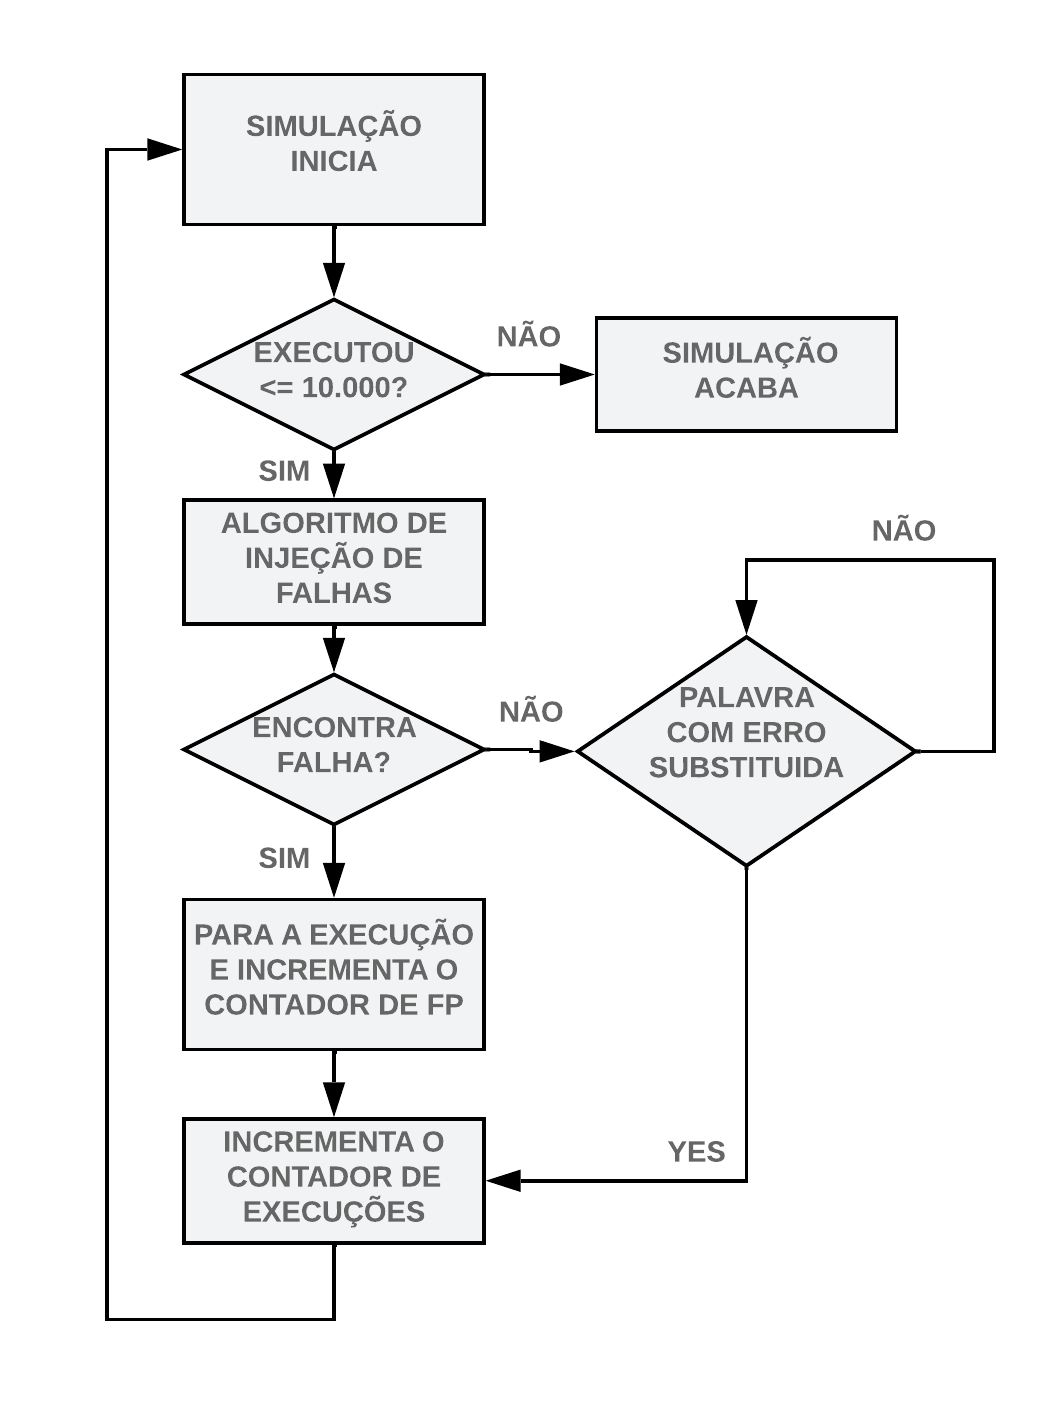
\includegraphics[scale=1]{modelo-dissertacao-ppgcc/figuras/algoritmo.png}
    \caption{Algoritmo da simulação}{Fonte: próprio autor}
    \label{fig:algoritmo}
\end{figure}

Antes de mostrar os resultados obtidos ao final do trabalho, a seção a seguir explica qual a abordagem proposta neste trabalho em adaptação ao código de \cite{sanchez2019reducing}.

\section{Esquema dos códigos propostos}
Este trabalho propõe utilizar uma diferente abordagem da codificação de \cite{sanchez2019reducing}, dessa vez, focando em grupos menores de bits por vez. Isso fica proposto devido ao princípio da localidade espacial, pois em endereços próximos apresenta-se maiores chances de acontecer uma combinação que gere falhas.

Foram propostos quatro cenários: utilizando os 4, 8, 12 e 16 bits mais à direita, ou seja, os menos significativos (LSB, do inglês \textit{least significant bit}), que é justamente onde ocorre a maioria dos falsos positivos.

O objetivo dos métodos propostos é verificar se os códigos seriam capazes de manter a mesma proteção contra falsos positivos que o código que utiliza todos os bits. Deste modo, se comprovado, poderia ter a mesma capacidade de proteção utilizando menos portas XOR, e consequentemente, menos área ocupada na implementação física. 

A Tabela 2 mostra o número de XORs dos cenários propostos em comparação com os do código original, para uma palavra de 32 bits. Como já foi dito anteriormente, a tabela evidencia que são necessárias 30 portas XOR para calcular as duas paridades (MSB e MSB-1) nesse cenário com 32 bits. Para fazer o mesmo com os 16 bits menos significantes, seria preciso 14 portas XOR. É possível notar que o número de portas XOR segue um padrão:
\begin{equation}
    N = B-2
\end{equation}
em que N é o número de portas e B é o número de bits que serão submetidos ao cálculo.

\begin{table}[ht]
\centering
\caption{Número de portas XOR para cada código proposto, comparado com o código original, para um exemplo com 32 bits}
\begin{tabular}{c|c|c|c|c|c}
\hline
\rowcolor[HTML]{EFEFEF} 
\textbf{Código }                            & \textbf{Original} & \textbf{4-LSB} & \textbf{8-LSB} &\textbf{ 12-LSB} & \textbf{16-LSB} \\ \hline
\cellcolor[HTML]{EFEFEF}Portas XOR & 30       & 2     & 6     & 10     & 14     \\ \hline
\cellcolor[HTML]{EFEFEF}\%         & 100      & 6,67  & 20    & 33,33  & 46,67  \\ \hline
\end{tabular}
\end{table}

A Figura \ref{fig:8lsb} exemplifica o circuitos de portas XOR no cenário que calcula os novos valores de MSB e MSB-1 utilizando apenas os 8-LSB, necessitando de 6 portas, reduzindo bastante os custos de implementação do física do código.

\begin{figure}[ht]
    \centering
    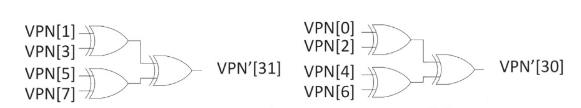
\includegraphics[scale=0.8]{figuras/8lsb.png}
    \caption{Circuito com as portas XOR no cenário de 8-LSB}{Fonte: adaptação de \cite{sanchez2019reducing}}
    \label{fig:8lsb}
\end{figure}

\section{Descrição dos experimentos}

O simulador desenvolvido para este trabalho, conta resumidamente com duas entradas e uma saída. Como mostrado na Figura \ref{fig:metod}, as entradas são os \textit{traces} de memória e o algoritmo de injeção de falhas, enquanto a saída é o número de falsos positivos obtidos naquela simulação. Os \textit{traces} simulam endereços de aplicações reais, que ocuparão as entradas da TLB. Como já foi dito, as aplicações testadas são: \textit{merge sort}, compressão, FFT e \textit{Bloom Filter}. A injeção de falhas insere três tipos de falhas nos bits dos endereços da TLB: erros simples, erros duplos adjacentes e erros triplos adjacentes.

\begin{figure}[ht]
    \centering
    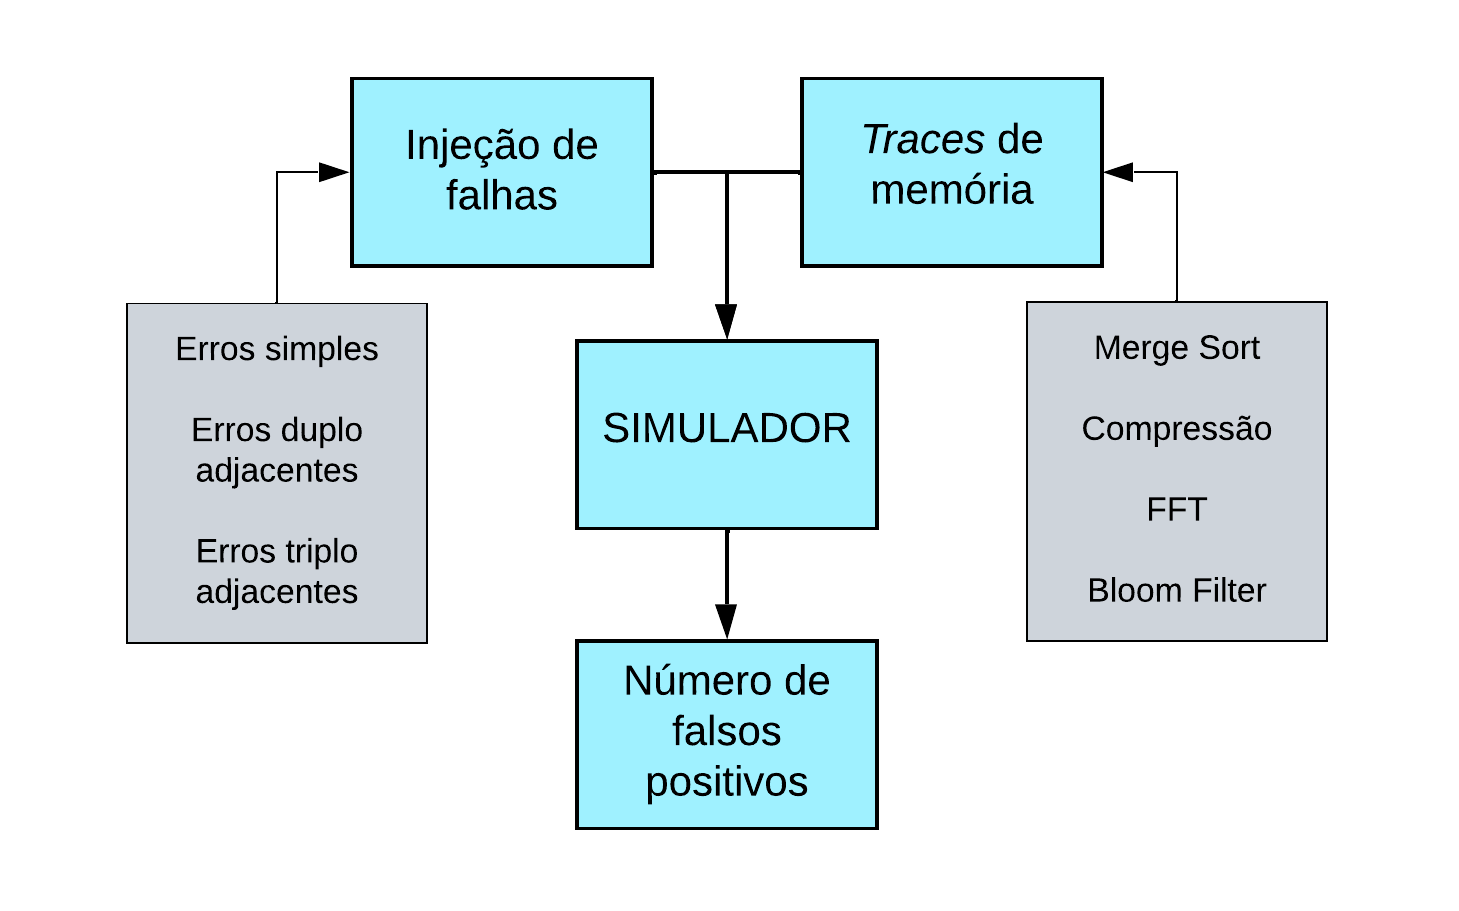
\includegraphics[scale=1]{modelo-dissertacao-ppgcc/figuras/metod.png}
    \caption{Diagrama com entradas e saída do simulador}{Fonte: próprio autor}
    \label{fig:metod}
\end{figure}

Ao fim de cada execução, o simulador retorna 1, para o caso de ter ocorrido falso positivo, ou 0, pro caso de não ter ocorrido. Essa saída é encaminhada para um contador que acumula esse resultado para todas as execuções do mesmo tipo (falha, código e \textit{trace}). 

Após obtidos os números de falsos positivos, esses valores foram convertidos em porcentagem, relacionando o resultado ao número total de execuções para cada cenário, ou seja, 10 mil. Essas porcentagens foram organizadas nas tabelas descritas no Capítulo 4.

\section{Conclusão}

Neste capítulo foi apresentada a metodologia empregada no desenvolvimento do trabalho. Além disso, foram descritos os experimentos realizados, a abordagem dos códigos propostos e as métricas de análise dos resultados. No Capítulo seguintes serão mostrados os resultados desses experimentos. 
\chapter{Resultados Preliminares}
\label{cap:resultados}

Neste capítulo serão apresentados os resultados dos experimentos detalhados no capítulo anterior. Os erros simples estão dispostos nas tabelas a seguir como SE, do inglês \textit{single errors}. Erros duplo adjacentes são os DAE, do inglês \textit{double adjacent errors}. E por fim, os erros triplos são os TAE, do inglês \textit{triple adjacent errors}.

\section{Discussão de Resultados}

A Tabela \ref{tab:noprotect} apresenta a porcentagem de falsos positivos obtidos nos experimentos para o cenário sem código de proteção. As falhas do tipo DAE resultaram em valores mais expressivos, apontando que a alteração em dois bits adjacentes aumentou a probabilidade de falsos positivos. Para o tipo de falha TAE, ocorre uma diminuição no contador de falsos positivos, provavelmente devido aos endereços com erros triplos apontarem para endereços distantes, resultando em falsos negativos.

\begin{table}[ht]
\centering
\caption{Porcentagem de falsos positivos para o cenário não protegido}
\begin{tabular}{
>{\columncolor[HTML]{EFEFEF}}c |c|c|c}
\hline
\textbf{Aplicação}    & \cellcolor[HTML]{EFEFEF}\textbf{SE(\%)} & \multicolumn{1}{l|}{\cellcolor[HTML]{EFEFEF}\textbf{DAE(\%)}} & \multicolumn{1}{l}{\cellcolor[HTML]{EFEFEF}\textbf{TAE(\%)}} \\ \hline
\textbf{Merge sort}   & 1,37                                    & 2,14                                                          & 1,79                                                         \\ \hline
\textbf{Compressão}   & 1,42                                    & 2,16                                                          & 1,73                                                         \\ \hline
\textbf{FFT}          & 1,26                                    & 1,98                                                          & 1,40                                                         \\ \hline
\textbf{Bloom Filter} & 1,22                                    & 2,37                                                          & 1,75                                                         \\ \hline
\end{tabular}
\label{tab:noprotect}
\end{table}

Os resultados da Tabela \ref{tab:fullprotect} indicam que o método de \cite{sanchez2019reducing} é bastante efetivo no tratamento de falsos positivos, evitando todos os erros nos três tipos de falha.


\begin{table}[ht]
\centering
\caption{Porcentagem de falsos positivos para o código proposto em \cite{sanchez2019reducing}}
\begin{tabular}{
>{\columncolor[HTML]{EFEFEF}}c |c|c|c}
\hline
\textbf{Aplicação}    & \cellcolor[HTML]{EFEFEF}\textbf{SE(\%)} & \multicolumn{1}{l|}{\cellcolor[HTML]{EFEFEF}\textbf{DAE(\%)}} & \multicolumn{1}{l}{\cellcolor[HTML]{EFEFEF}\textbf{TAE(\%)}} \\ \hline
\textbf{Merge sort}   & 0                                       & 0                                                             & 0                                                            \\ \hline
\textbf{Compressão}   & 0                                       & 0                                                             & 0                                                            \\ \hline
\textbf{FFT}          & 0                                       & 0                                                             & 0                                                            \\ \hline
\textbf{Bloom Filter} & 0                                       & 0                                                             & 0                                                            \\ \hline
\end{tabular}
\label{tab:fullprotect}
\end{table}

A Tabela \ref{tab:my} apresenta os resultados para os cenários onde apenas os LSBs são utilizados para o cálculo das paridades, propostos neste trabalho. Para os cenários de 8- a 16-LSB, os resultados são similares aos obtidos com o método original. Para 4-LSB foi percebida uma redução considerável no número de falsos positivos. Por exemplo, para a aplicação do \textit{Merge Sort}, o número de falsos positivos é reduzido a 17\%\ para SE e 10\%\ para DAE e TAE.

\begin{table}[ht]
\centering
\caption{Porcentagem de falsos positivos para cada cenário proposto}
\begin{tabular}{
>{\columncolor[HTML]{EFEFEF}}l |
>{\columncolor[HTML]{EFEFEF}}l |c|c|c}
\hline
\textbf{Aplicação}                                     & \cellcolor[HTML]{EFEFEF}\textbf{Cenário} & \multicolumn{1}{l|}{\cellcolor[HTML]{EFEFEF}\textbf{SE(\%)}} & \multicolumn{1}{l|}{\cellcolor[HTML]{EFEFEF}\textbf{DAE(\%)}} & \multicolumn{1}{l}{\cellcolor[HTML]{EFEFEF}\textbf{TAE(\%)}} \\ \hline
\cellcolor[HTML]{EFEFEF}                               & \cellcolor[HTML]{EFEFEF}4-LSB            & 0,24                                                         & 0,21                                                          & 0,17                                                         \\ \cline{2-5} 
\cellcolor[HTML]{EFEFEF}                               & \cellcolor[HTML]{EFEFEF}8-LSB            & 0                                                            & 0                                                             & 0                                                            \\ \cline{2-5} 
\cellcolor[HTML]{EFEFEF}                               & \cellcolor[HTML]{EFEFEF}12-LSB           & 0                                                            & 0                                                             & 0                                                            \\ \cline{2-5} 
{\cellcolor[HTML]{EFEFEF}\textbf{Merge sort}}    & \cellcolor[HTML]{EFEFEF}16-LSB           & 0                                                            & 0                                                             & 0                                                            \\ \hline
\cellcolor[HTML]{EFEFEF}                               & 4-LSB                                    & 0,21                                                         & 0,31                                                          & 0,27                                                         \\ \cline{2-5} 
\cellcolor[HTML]{EFEFEF}                               & 8-LSB                                    & 0                                                            & 0                                                             & 0                                                            \\ \cline{2-5} 
\cellcolor[HTML]{EFEFEF}                               & 12-LSB                                   & 0                                                            & 0                                                             & 0                                                            \\ \cline{2-5} 
{\cellcolor[HTML]{EFEFEF}\textbf{Compressão}}   & 16-LSB                                   & 0                                                            & 0                                                             & 0                                                            \\ \hline
\cellcolor[HTML]{EFEFEF}                               & 4-LSB                                    & 0,31                                                         & 0,19                                                          & 0,24                                                         \\ \cline{2-5} 
\cellcolor[HTML]{EFEFEF}                               & 8-LSB                                    & 0                                                            & 0                                                             & 0                                                            \\ \cline{2-5} 
\cellcolor[HTML]{EFEFEF}                               & 12-LSB                                   & 0                                                            & 0                                                             & 0                                                            \\ \cline{2-5} 
{\cellcolor[HTML]{EFEFEF}\textbf{FFT}}          & 16-LSB                                   & 0                                                            & 0                                                             & 0                                                            \\ \hline
\cellcolor[HTML]{EFEFEF}                               & 4-LSB                                    & 0,34                                                         & 0,28                                                          & 0,17                                                         \\ \cline{2-5} 
\cellcolor[HTML]{EFEFEF}                               & 8-LSB                                    & 0                                                            & 0                                                             & 0                                                            \\ \cline{2-5} 
\cellcolor[HTML]{EFEFEF}                               & 12-LSB                                   & 0                                                            & 0                                                             & 0                                                            \\ \cline{2-5} 
{\cellcolor[HTML]{EFEFEF}\textbf{Bloom Filter}} & 16-LSB                                   & 0                                                            & 0                                                             & 0                                                            \\ \hline
\end{tabular}
\label{tab:my}
\end{table}

Em todas as aplicações do \textit{benchmark}, os resultados apontam que a maioria dos erros que geram falsos positivos acontecem se concentram nos bits menos significativos, e verificam que é possível proteger a i-TLB com um método simples e reduzindo o número de portas XOR usadas no circuito. 

\section{Conclusão}

SEUs e MCUs podem causar falsos positivos em i-TLBs gerando falhas graves como congelamento do sistema e corrupção silenciosa de dados. Os métodos para proteger os i-TLBs geralmente são baseados em bits de redundância e adicionam sobrecarga de área. Um código baseado apenas em paridade e sem bits extras é capaz de reduzir o número de falsos positivos. Neste trabalho, estendemos este código explorando ainda mais o princípio da localidade. Propomos calcular a paridade dos LSBs, pois erros nesses bits são mais propensos a causar falsos positivos do que erros nos bits superiores. Os resultados apontam que os cenários com 8-, 12- e 16-LSBs atingem níveis de proteção equivalentes ao código original. Além disso, o cenário com 4 LSBs também apresenta um bom desempenho.
 


% ----------------------------------------------------------
% Finaliza a parte no bookmark do PDF
% para que se inicie o bookmark na raiz
% e adiciona espaço de parte no Sumário
% ----------------------------------------------------------
\phantompart

% ---
% Conclusão
% ---
\chapter{Cronograma de Atividades}
% ---
A tabela a seguir mostra o cronograma mensal previsto de atividades a serem realizadas a partir da qualificação até a defesa da dissertação. Continuidade nos experimentos se refere a testar a abordagem deste trabalho em alguns dos códigos apresentados na Fundamentação Teórica, além de verificar os resultados para uma TLB com mais posições de entrada.

Em fevereiro foi submetido um artigo à \textit{20th  IEEE International New Circuits and Systems Conference} (NEWCAS), cujo resultado da aprovação será em Abril. Espera-se obter novos resultados para submeter novo artigo ao \textit{Symposium on Integrated Circuits and Systems Design} (SBCCI) 2022.

É interessante implementar os códigos propostos em Linguagem de Descrição de Hardware (HDL, do inglês \textit{Hardware Description Language}), e a partir daí realizar testes de área e potência. Por fim, após testar outros códigos e obter resultados mais precisos sobre as vantagens de se proteger apenas os bits necessários, finalizar o texto da dissertação. O objetivo é defender a dissertação ao final do mês de Agosto.

\begin{table}[ht] 
\centering
\caption{Cronograma mensal de atividades}
\begin{tabular}{
>{\columncolor[HTML]{EFEFEF}}l |c|c|c|c|c|c}
\hline
\textbf{Atividade}     & \multicolumn{1}{l|}{\cellcolor[HTML]{EFEFEF}\textbf{mar}} & \multicolumn{1}{l|}{\cellcolor[HTML]{EFEFEF}\textbf{abr}} & \multicolumn{1}{l|}{\cellcolor[HTML]{EFEFEF}\textbf{mai}} & \multicolumn{1}{l|}{\cellcolor[HTML]{EFEFEF}\textbf{jun}} & \multicolumn{1}{l|}{\cellcolor[HTML]{EFEFEF}\textbf{jul}} & \multicolumn{1}{l}{\cellcolor[HTML]{EFEFEF}\textbf{ago}} \\ \hline
Defesa da qualificação    & x                                                         &                                                           &                                                           &                                                           &                                                           &  \\
\hline
Continuidade nos experimentos    & x                                                         &    x                                                       &                                                           &                                                           &                                                           &  \\\hline
Resultado da submissão no NEWCAS     &                                                          & x                                                         &                                                           &                                                           &                                                           &                                                                                                                 \\ \hline
Submissão de trabalho no SBCCI 2022     &                                                          & x                                                         &                                                           &                                                           &                                                           &                                                          \\ \hline
Implementação dos códigos em HDL  &                                                           &                                                          & x                                                         &                                                           &                                                           &                                                           \\ \hline
Testar implementação em simulador de FPGA   &                                                           &                                                           & x                                                         &    x                                                       &                                                           &                                                          \\ \hline
Resultados em área e potencia   &                                                           &                                                           &                                                           & x                                                         &                                                           &                       \\ \hline
Revisão da dissertação &                                                           &                                                           &                                                           &                                                           & x                                                         &                                                          \\ \hline
Defesa da dissertação              &                                                           &                                                           &                                                           &                                                           &                                                           & x                                                        \\ \hline
\end{tabular}
\end{table} 				% Capítulo de introdução

% ----------------------------------------------------------
% ELEMENTOS PÓS-TEXTUAIS
% ----------------------------------------------------------
\postextual
% ----------------------------------------------------------

% ----------------------------------------------------------
% Referências bibliográficas
% ----------------------------------------------------------
\bibliography{referencias}

% ----------------------------------------------------------
% Glossário
% ----------------------------------------------------------
%
% Consulte o manual da classe abntex2 para orientações sobre o glossário.
%
%\glossary

% ----------------------------------------------------------
% Apêndices
% ----------------------------------------------------------

% ---
% Inicia os apêndices
% ---
%\begin{apendicesenv}

% Imprime uma página indicando o início dos apêndices
%\partapendices
% Insere os apêndices
%% ----------------------------------------------------------
\chapter{Nullam elementum urna vel imperdiet sodales elit ipsum pharetra ligula
ac pretium ante justo a nulla curabitur tristique arcu eu metus}
% ----------------------------------------------------------
\lipsum[55-57]
%\chapter{Quisque libero justo}
% ----------------------------------------------------------

\lipsum[50]
%\include{apendices/apendice-c}
%\include{apendices/apendice-d}




%\end{apendicesenv}
% ---


% ----------------------------------------------------------
% Anexos
% ----------------------------------------------------------

% ---
% Inicia os anexos
% ---
%\begin{anexosenv}

% Imprime uma página indicando o início dos anexos
%\partanexos
% Insere os anexos
%\chapter{Morbi ultrices rutrum lorem.}
% ---
\lipsum[30]

%\chapter{Cras non urna sed feugiat cum sociis natoque penatibus et magnis dis
parturient montes nascetur ridiculus mus}
% ---

\lipsum[31]
%\include{anexos/anexo-c}
%\include{anexos/anexo-d}

%\end{anexosenv}

%---------------------------------------------------------------------
% INDICE REMISSIVO
%---------------------------------------------------------------------
\phantompart
\printindex
%---------------------------------------------------------------------

\end{document}
